        % ****** Start of file apssamp.tex ******
%
%   This file is part of the APS files in the REVTeX 4.1 distribution.
%   Version 4.1r of REVTeX, August 2010
%
\documentclass[reprint,%article
 %,
%superscriptaddress,
%groupedaddress,
%unsortedaddress,
%runinaddress,
%frontmatterverbose, 
%preprint,
%showpacs,preprintnumbers,
%nofootinbib,
%nobibnotes,
%bibnotes,
 amsmath,amssymb,
 aps,
%pra,
%prb,
%rmp,
%prstab,
%prstper,
%floatfix,
]{revtex4-1}
\usepackage[table,xcdraw]{xcolor}

%\usepackage{xcolor}

\usepackage{graphicx}% Include figure files
\usepackage{dcolumn}% Align table columns on decimal point
\usepackage{bm}% bold math
\usepackage{appendix}
\usepackage{subcaption}
\usepackage[a4paper,margin=10mm,includefoot]{geometry}
\usepackage{array,ragged2e,longtable}
\newcolumntype{P}{>{\RaggedRight\hspace{0pt}}p{\dimexpr(\textwidth-1cm -10\tabcolsep -5\arrayrulewidth)/4\relax}}

%\usepackage{subfloat}
%\usepackage{hyperref}% add hypertext capabilities
%\usepackage[mathlines]{lineno}% Enable numbering of text and display math
%\linenumbers\relax % Commence numbering lines

%\usepackage[showframe,%Uncomment any one of the following lines to test 
%%scale=0.7, marginratio={1:1, 2:3}, ignoreall,% default settings
%%text={7in,10in},centering,
%%margin=1.5in,
%%total={6.5in,8.75in}, top=1.2in, left=0.9in, includefoot,
%%height=10in,a5paper,hmargin={3cm,0.8in},
%]{geometry}https://www.overleaf.com/project/5ba0361831a91c7b3990c0d7
 \usepackage{natbib}
 
\begin{document}

\preprint{APS/123-QED}

\title{DRAFT- Rotation Curve Fitting Model }% Force line breaks with \\
%\thanks{ Thanks Jesus}%

% Find out if Joe and Noah still want to be on this paper%

 

\author{Sophia Natalia Cisneros}
 \affiliation{ Department of Astronomy,  
 University of Washington}
 % \email{sophia.cisneros@du.edu}
  \author{Richard Ott}%
 \email{rich.ott@EMAIL.com}
\affiliation{Affiliate MIT - Ask Joe }%Tech dudes \textbackslash\textbackslash
%}
 \author{ Meagan Crowley}
\email{ }
\affiliation{NREL, School of Mines}%
 \author{ Amy Roberts}
\email{ }
\affiliation{CU Denver}%
\author{Marcus Paz}
\author{Zaneeyiah Brown}
\author{Landon Joyal}
\author{Roberto Real Rico}
\author{Elizabeth Gutierrez-Gutierrez}
\author{ Phong Pham}
\author{Zac Holland}
\author{Amanda Livingston}
\author{Lily Castrellon}
\author{Shanon Rubin}
\author{Aaron Ashley}
\author{Dillon Battaglia}
%\affiliation{UMass Boston% with \\
%&}%
%
 
 
\date{\today}% It is always \today, today,
             %  but any date may be explicitly specified
             %%%%%%
%%%%%%%
%%%%%%
%%%%%%%
%%%%%%
%%%%%%%
\begin{abstract}
 
 
{\color{teal}   Github repo: Cisneros-Galaxy/RCFM     }

\begin{description}
\item[Usage]
Secondary publications and information retrieval purposes.
\item[PACS numbers]
May be entered using the \verb+\pacs{#1}+ command.
%\item[Structure]
%You may use the \texttt{description} environment to structure your abstract;
%use the optional argument of the \verb+\item+ command to give the category of each item. 
\end{description}
\end{abstract}

\pacs{Valid PACS appear here}% PACS, the Physics and Astronomy
                             % Classification Scheme.
%\keywords{Suggested keywords}%Use showkeys class option if keyword
                              %display desired
\maketitle

%\tableofcontents
%%%%%%NOTES TO DO
%%%make labels for figure axes. remove orange line through the data
%%%%%%
%%%%%%%%
%%%%%%
%%%%%%%
%%%%%%
%%%%%%
\section{Introduction  \label{sec:uno}}


%DARK MATTER

  At the level of the data, the flat-rotation curve problem of spiral galaxies is  the divergence of two velocity parameters that come  from  different    observations of total light
 \cite{Rub,Bosma,1985ApJAlbada}. 
 The  observations   are photometry and Doppler shifted spectra. 
 Photometry is a measure of total light, which when associated with luminous mass, 
 gives Keplerian velocities through a
Poisson  dynamics.  
The Keplerian orbital  velocities   descend  past   the stars. 
The counter observable is frequency treated by a Lorentz  Doppler shift formalism to give   rotation curve velocities. 
The rotation curve velocities remain ``flat''  far past the stars (see Fig.~\ref{fig:NGC2403RCFM}). The divergence of these velocity parameters is   known as the 
  flat-rotation curve problem, and  is
 primary evidence for dark matter.

 
In the dark matter paradigm   both   Keplerian  and the rotation curve velocities are  proxies for mass,  and so their divergence signals a   missing or ``dark'' matter component in these systems . 
Dark matter theories are built to be consistent with standard Einstein gravity, though      comprised of new dark particles  which augment the standard model. The  dark matter  particles are hypothesized to    have a very low interaction probability with baryonic matter, and so   direct detection experiments are ever increasing levels of sensitivity  to find them \cite{Cebrian:2022brv}. However, in the absence of  direct detection,   the paradoxes of dark matter theory remain    interesting.   
 
 

 
   \begin{figure}[h!] 
    \begin{subfigure}[c]{0.95\linewidth}
    \centering
    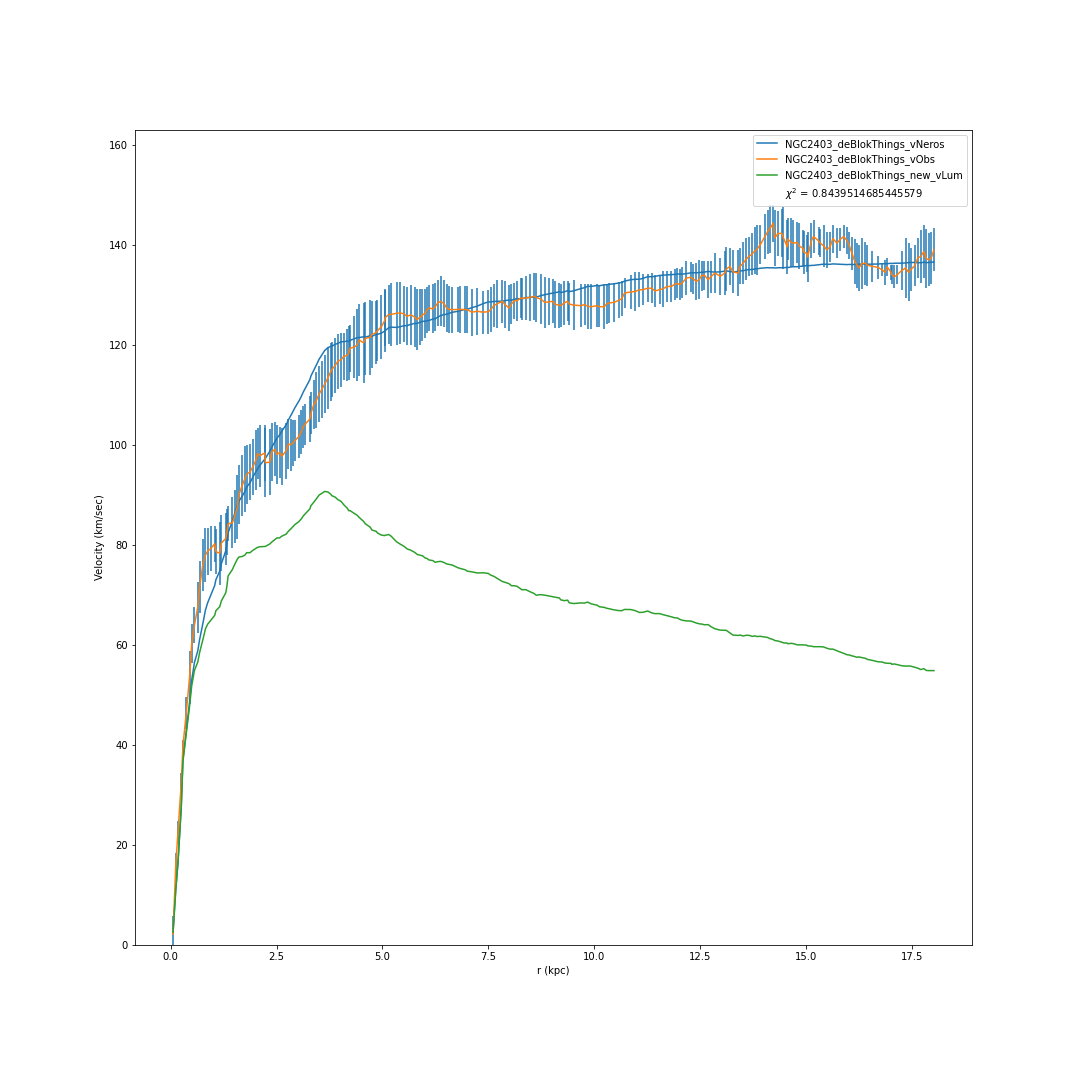
\includegraphics[width=0.95\linewidth]{figures/NGC2403_deBlokThings_XueSofue}
   % \caption{ }
  \end{subfigure}%%
  \caption{ RCFM fit to  NGC 2403  rotation curve data and   baryon model from  \citet{Blok1})}  \label{fig:NGC2403RCFM} 
\end{figure}



  S. McGaugh  notes one such paradox when he asks   ``Why is the luminous tail wagging the dark matter dog,  if dark matter dominates dynamics ?'' \cite{1999McGaugh,McGaugh2016RAR}. This references the  curious fact   that knowledge  of 
 the   stellar   disk   completely  determines the spherical dark matter halo \cite{2004ApJ...609..652M}. A   related paradox is the Universal Rotation Curve (URC), which is a spectrum of   1,100  rotation curves normalized by scale-length and plotted on the same axes 
 (See Fig.~\ref{fig:URC})  \cite{salucci,Persic,1978Rubin,10.1111/j.1365-2966.2007.11696.x}. The URC spectrum   inflects about a median point of truly flat rotation curves which are coincidentally where the Milky Way's presumed rotation curve lies.  Further,  galaxies larger than the Milky Way have 
 rotation curves which    inflect down towards the   flat, and those galaxies smaller than the Milky Way have rotation curves which inflect up towards flat.
 In the dark matter paradigm there is no explanation for  this phenomenon \cite{MCGAUGH2021220}. We will instead interpret the URC spectrum as indicative of   a frame-dependency due the Milky Way in what follows. 

 
   
 \begin{figure}[h!]
     \centering
     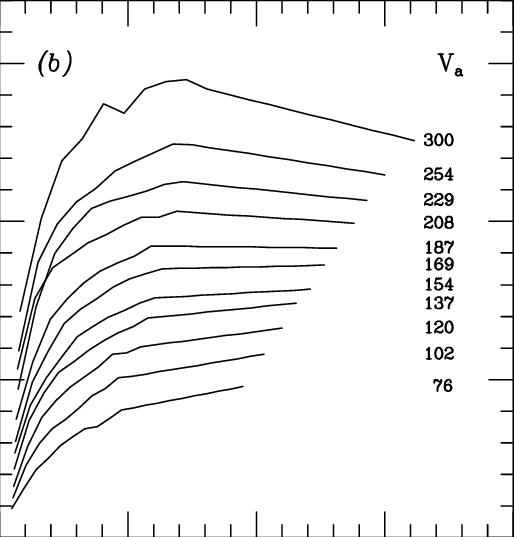
\includegraphics[width=\linewidth]{The-universal-rotation-curve-of-spiral-galaxies-at-different-luminosities-and-velocities}
     \caption{Universal Rotation Curve spectrum from Ref.\citep{salucci}. Used with permission}
     \label{fig:URC}
\end{figure}
  

    


% This paradox    requires fundamental modifications to the classical theory of gravity, because in classical gravity mass accretion rates favor   larger mass concentrations \cite{10.1093/mnras/stt2403}.  However,    these paradoxes disappear if we instead view them as indicative of  frame dependent effects due to  the relative frame of the   Milky Way, imprinted on observations of Doppler shifted spectra. 
 
The   leading   alternative     to dark matter  is   Modified Newtonian Dynamics (MOND) \cite{Milgrom},  in which     the   luminous mass is the only mass   but  there is   a changing   scale of gravitational acceleration to explain the flat-rotation velocities  \cite{McGaugh_2014}. MOND introduces a new acceleration scale to successfully fit   a large number of spiral galaxies  rotation curves with essentially a single, constant acceleration scale \cite{2016Lelli}.   But, while MOND removes the problem of dark matter from these systems efficiently, it still remains a   fundamental  alteration of   physics, which when extended  to the relativistic regime   gives rise to  new theories of gravity  \cite{PhysRevD.70.083509,doi:10.1142/S0217751X0703666X,Famaey2012}.


We  will instead approach this problem in  more conservative way,  which does not  modify physics. By considering the problem at the level of the data, we interpret excesses in Doppler shifted spectra not as physical rotation velocities but rather as relative gravitational frame effects due to our Milky Way.  This transitions   MOND's  changing acceleration scale to the relativistic concept of    relative galaxy  curvatures. 
The rotation curve fitting model (RCFM)  presented here    preserves the fitting successes of MOND and dark matter models, but   improves upon   some notorious problem galaxies.   We demonstrate     the efficiency of the RCFM approach by fitting   the SPARC sample of 175 galaxy rotation curves  previously   fitted by the MOND, dark matter models, and the    RAR (Radial Acceleration Relation) \cite{McGaugh2016RAR,2016Lelli,McGaugh_2014,Li_2018}. 


  Previously, the role of relative
     galaxy curvature  in this problem was obviated 
       by  Galilean subtraction of   gravitational red-shifts at the  large $r$  limit of the data \citep{MTW}.   At this time, there are many problems in   the concordance model of   cosmology which are attributed to dark matter \cite{2010dmp..book.....S,Tully:2014gfa,Naidu_2022}, but in
 this paper we address only this  one, as it is the simplest. 

 
 This paper  is organized as follows;
{\bf Section \ref{sec:dos}} constructs  the new rotation curve  fitting formalism, 
{\bf Section \ref{sec:data}}   describes  the data  we use, 
 {\bf Section \ref{sec:analysis}}   discusses our results, 
 and  {\bf Section \ref{sec:conclu}}   discusses implications and future tests.   
  

  
    

%%%%%%
%%%%%%%%
%%%%%%
%%%%%%%
%%%%%%
%%%%%%
\section{ Rotation Curve Fitting Models  \label{sec:dos}}
 
 
 \subsection{Dark matter rotation curve fitting formula}
 
  

 The   dark matter rotation curve formula   is of the form

 \begin{equation}
v(r)^2_{rot}  =  v(r)^2_{lum}  +  v(r)^2_{dm},   
\label{eq:zonte1}
\end{equation} 

  where terms in $v(r)_{lum}$ are the Keplerian velocities from estimates of   luminous mass,  $v(r)_{dm}$ are the velocities attributed to  dark matter, and 
  terms in $v(r)_{rot} $ are the dark matter  predictions,  which are fitted to the flat rotation curve data
  $v_{obs}(r)$. All velocities are assumed to be those of test particles in circular orbits, in the plane of the stellar disk,  about the rotation axis of the galaxy at  $r=0$. 
  

The flat rotation curve velocity parameters    $v_{obs}(r)$  come from an inertial 
 Lorentz boost  of  observed  Doppler shifted spectra data  $\omega'(r)$,  
   

 \begin{equation}
 \frac{v_{obs}(r) }{c}=
\frac{  \left( \frac{\omega'(r)}{\omega_o}\right)^2 -  \left( \frac{\omega_o}{\omega'(r)} \right)^2 }{  \left( \frac{\omega'(r)}{\omega_o}\right)^2  +  \left( \frac{\omega_o}{\omega'(r)}\right)^2 }, 
\label{eq:modelLumA}
\end{equation} 

  where the    $\omega_o$  are the
  characteristic lab  frame frequencies for some well-known atomic transitions, and terms in $c$ are  the constant vacuum light speed. 

  
  
  
 %%%%%%%%%%%%%%%%%
 %%%%%%%%%%%%%%%%%%
%%%%%%%%%%%%%%%%%%%%
  Keplerian velocities due to   luminous mass $v_{lum}$ (Eq.~\ref{eq:zonte1})
   come from associating  baryonic  mass with observations of total light  (photometry)  through  population synthesis models (PSM).  
  These mass distributions are    used to 
  calculate the Newtonian gravitational potential  
\begin{equation}
      \Phi(r)  = -G \int d^3r'  \frac{ \rho(r') }{r-r'}.
      \label{eq:Newt}
      \end{equation}
  
which solves Poisson's equation

\begin{equation}
\nabla^2 \Phi(r)_{lum}  = 4\pi G \rho(r),     
    \label{whatsgood}
\end{equation}

   terms in  $G$   are  Newton's   gravitational constant, and 
$\rho(r')$ is the mass density per unit volume. 
The gradient of the potential    yields the circular orbital velocities $v_{lum}$ (Eq.~\ref{eq:zonte1}) by

\begin{equation}
 \frac{\partial \Phi(r)_{lum}}{\partial r}    =\frac{v(r)_{lum}^2}{r}.  
    \label{zoochance1}
\end{equation}

  

The baryonic components of disk   galaxies include stellar bulge, stellar disk, and a gas halo
  
   \begin{equation}
v(r)_{lum}^2 = \gamma_b v(r)_{bulge}^2 +  \gamma_d v(r)_{disk}^2 + v(r)_{gas}^2.  
\label{eq:zonte3}
\end{equation} 
  
Terms in mass-to-light ratios $\gamma_b$ and $\gamma_d$ are   for the stellar bulge and for the stellar disk      respectively. 
  Gas fractions $v_{gas}$ are calculated from surface density profiles of HI  with the formalism given in  \cite{1983MNRAS.203..735C}, and do not require  a mass-to-light ratio.  
  
 


\subsection{New rotation curve fitting model (RCFM)}

We resolve the dark matter    paradoxes    by  attributing excesses in Doppler shifted spectra to  a gravitational frame-dependency  due to our Milky Way, not to excesses in rotation velocities.  
The   RCFM  
replaces the dark matter term $v(r)^2_{dm}/r$,  representing the gradient in the gravitational potential,       with  Lorentz-type mapping between the extended gravitational frames of galaxies, one-to-one in radius.  Like MOND, we   assume baryonic mass is the only mass. 


Fundamental to this approach is the   identification of  luminosity   as a Lorentz scalar, and Doppler shifted spectra as part of a 4-vector. Lorentz scalars are agreed upon by both frames, under a reliable distance indicator  (Cepheid variable stars, Tip of the Red Giant Branch), and 4-vectors transform in a Lorentzian sense.  
We   will also assume for convenience,  that the contributions to  Doppler shifted spectra from  relative frame  motion ($v_{lum}$) can be  separated from those from relative curvature roughly as in Eq.~\ref{eq:zonte1} \cite{Jack,Cisn}.  


 
 
   
   The RCFM we find it
   

\begin{equation}
v(r)_{rc}^2 =  v(r)_{lum}^2+\alpha \kappa^2 v(r)_{1} v(r)_{2},  
\label{eq:zonteLCM}
\end{equation}  

for $v(r)_{rc}$ the model's prediction which is fitted to $v_{obs}$, terms in $v_{lum}$ remain   as in 
  Eq.~\ref{eq:zonte1}, and the   term   replacing  dark matter is  $\alpha \kappa^2 v(r)_{1} v(r)_{2}$. This term is a product of the model's free fitting parameter $\alpha$, a curvature ratios ($\kappa$),  and two Lorentz-type transformation $v_1$ and $v_2$. 
  In what follows we will drop explicit representation of functional dependence on $r$, and so all   terms  can be assumed to  be functions of radius except the model's free parameter $\alpha$,  which is single valued for each galaxy fitted, and other constants like the lab-frame frequency $\omega_o$, Newton's constant $G$ and the speed of light $c$.  
  
  Terms in 
$\kappa$  are   ratios of the baryonic gravitational potentials 

 \begin{equation}
\kappa=\frac{\Phi_{gal}}{\Phi_{mw}}, 
\label{eq:kappa2}  
\end{equation}  

 for $\Phi_{gal}$ the    Newtonian gravitational potential of the galaxy being observed, and $\Phi_{mw}$ that of  the Milky Way.  
 
 
 To characterize    excesses in Doppler shifted spectra
  as     part of  a Lorentz 4-vector, we have investigated the space of hyperbolic transformations  \cite{Cisneros:2013vha,Cisneros:2014fea,Cisneros2015,Cisn2016}, and found the best fit function for $v_1$ to be

 
 
   \begin{equation}
       v_1 = \sinh \zeta, 
       \label{eq:hyperbolica}
   \end{equation}
 
 for a rapidity angle $\zeta$  defined by the    Lorentz exponential  term  
  
   
     \begin{equation}
     e^{\zeta}=  \frac{\omega_{mw}}{\omega_{gal}}  =\sqrt{\frac{g_{tt}|_{gal}}{g_{tt}|_{mw}}}.
      \label{eq:gravRS}
    \end{equation}
    
 The clock terms $g_{tt}$  are the time components of the  Schwarzschild metric.  They are defined in the   weak field limit  \cite{Hartle} as, 
 
  \begin{equation}
      g_{tt}= -( 1 - 2\Phi/ c^2).
      \label{clocktime}
  \end{equation} 
  

The best   function we find  for  $v_2$ is 

\begin{equation}
v_{2} =  \cosh \tau, 
\label{eq:hyperbolico}
\end{equation}

 for the rapidity angle $\tau$ defined by the    Lorentz exponential  term  
  
 
\begin{equation}
    e^{\tau}=   e^{(\zeta+\eta)/2}.
\end{equation}
 
Terms in $e^{\tau}$ are  convolutions of the curved 2-frame $e^\zeta$ (Eq.~ \ref{eq:gravRS})  with flat 2-frame $e^\eta$ where observations are made.  That this second transformation  is necessary is evidenced by the local constancy of the speed of light, ie. the equivalence principle. 

  The flat field frames  are represented by the
Lorentz exponential  

\begin{equation}
    e^{\eta}=\frac{\omega_{l}}{\omega_o}= \sqrt{\frac{1+\beta}{1-\beta}},
    \label{eq:flat}
\end{equation}  
     
for $\beta = v_{lum}/c$. 
Frequency shifts $\omega_{l}$ are those expected   
in a flat spacetime for a relative frame velocity   $v_{lum}/c$, 
as in Eq.~\ref{eq:modelLumA}.  
Use of Eq.~\ref{eq:flat} asserts  that Keplerian rotation curves are     the best estimate of flatness, since dark matter is not required to  reproduce the rotation curve of our Solar System.
 
  Lorentz exponential terms (Eq.~\ref{eq:gravRS} and Eq.~\ref{eq:flat})
  are    identified  as the  frame field relationships   by  comparison of 
     the inertial frame Lorentz transformation in  Eq.~\ref{eq:modelLumA} with 
the  hyperbolic form \cite{rindler2013essential} 


     \begin{equation}
         \frac{v}{c} = \tanh \theta = \frac{e^\theta - e^{-\theta}}{e^\theta + e^{-\theta}} .   
         \label{boost}
     \end{equation} 

 
 
  
  Viewed as    Rindler's accelerated coordinates\cite{MTW,Wald, rindler2013essential}, 
     $v_1$   is  timelike   and $v_2$ is spacelike. This is a heuristic construction only, though one may assume that if the RCFM proves a physical model for rotationally supported galaxies, then a fundamental derivation must exist. 

 
    
 
%%%%%%
%%%%%%%
%%%%%%
%%%%%%%  
%%%%%%
%%%%%%%  
\subsection{Synchronizing the gravitational potentials \label{sec:gravDets}}

  


 
The RCFM  terms in  $v_1$ and $v_2$ are parametrized with ratios of  the    Schwarzschild gravitational clock terms. These come from the gravitational redshift formula

\begin{equation}
       \frac{\omega_1}{\omega_2}  =\sqrt{\frac{g_{tt}|_{P2}}{g_{tt}|_{P1}}} =\sqrt{\frac{|\xi^t\xi_{t}|_{P2}}{|\xi^t\xi_{t}|_{P1}}},
      \label{eq:grav}
    \end{equation} 
    
which    gives the change in  photon energy  from point $P1$ to $P2$ in a single, simply connected gravitational   manifold \cite{Wald}.  The gravitational redshift formula Eq.~\ref{eq:grav} is derived from the conservation properties of the Killing vector field.  The norm of the timelike Killing field in a Schwarzschild spacetime is $\sqrt{g_{tt}}$, which   is  parametrized with the Newtonian gravitational potential as per
    Eq.~\ref{clocktime}. 


 The equivalence principle requires that locally all frames are inertial, and so special relativity applies.  ``Thus, when going from
one local inertial frame at a given point to another at the same point, the fields transform
with respect to a Lorentz transformation ''\cite{jetzer}(tetrad formalism). To extend  Eq.~\ref{eq:grav} to  relate two distinct manifolds at the same radii,    our first step is to make galaxies inertial frames.   To  do so, we consider  Wolfgang Rindler's statement that        ``the center of each galaxy provides a basic local standard of nonacceleration ... so then can be treated like a local inertial frame relative to its own center.''\cite{rindler2013essential}.
    We identify this to mean that  to make galaxies inertial frames with respect to each other, we must synchronize their centers. 
    
    
  
  Usually,   gravitational potentials of galaxies   are integrated  from the large $r$ limit into the smallest $r$ 
  as in Eq.~  \ref{eq:Newt}. At the large $r$ limit      the potential is assumed  to go to zero,   to ensure a  globally  flat embedding space where energy goes to zero at infinity. 
  However,    it appears that to recover energy conservation one must assess the system at  significantly larger scales than galaxies.
 At the present time,  observations of  the local environments of galaxies show highly complex streamlines \cite{Pomarede:2020pme,Hoffman:2017ako}. 
 We drop the constraint of a flat embedding space, and  instead integrate all    potentials    from a different  zero, namely  at the galactic center $r\approx 0$, so   we   compare galaxies as inertial frames using Lorentz-type boosts, and because at the event horizon $R_s$   all clocks read  zero   $g_{tt} \to 0$.

 Reversing the usual integration order 
 
  \begin{equation}
     \Phi  =    \int_{inner}^{outer} \vec{F_r}\cdot\vec{dr}, 
      \label{eq:Newt2}
      \end{equation}
      
for $F_r = v^2/r$ the force per unit mass, produces gravitational 
potentials based on    Killing vector fields which are aligned with the rotation centers of galaxies. In this way, we use  Eq.~\ref{eq:grav}  to relate two points $P1$ and $P2$ in two
distinct galaxy manifolds, one-to-one in  radii.  
 Reversing the integration order    in this way produces potentials which still obey Poisson's equation Eq.~\ref{whatsgood} and the central force law Eq.~\ref{zoochance1}.

 
\subsection{  Geometry Considerations  }\label{GeomSphere}
  
   Population synthesis models commonly assume spherical symmetry for the 
  stellar bulge, gas halo, but   axial symmetry for    the stellar disk \cite{1954AJ.....59..273S,Freeman}.
 However, it is a common calculational  tool to use spherical symmetry for the entire integrated potential of the luminous mass distribution  \cite{2022A&A...664A..40M,PhysRevD.70.083509}, because numerical integration of the thin disk is  computationally intensive,  requires assumptions of  boundary conditions,   relevant physical scales,  etc., and therefore adds extra free parameters to the problem \cite{2011A&A...531A..36H}.  
 We   use the spherical approximation   for the above reason and also,   the simplest metric for this situation is  
 Schwarzschild. We have previously tested use of the Kerr metric in this problem, and the   differences from what is stated in this paper are below the   observational limits \cite{Cisn}. 
 
Gravitational potentials calculated for  a spherically symmetric  geometry   
  merge to those calculated for an exponential disk  at lengths greater than one-third of the exponential scale-length of the disk $R_e$, ie.  $r> R_e/3$\cite{Chatterjee}. This is the region  where dark matter effects becomes important \cite{1985ApJAlbada}. 
However, 
    in the inner region of a galaxy $r< R_e/3$,  the spherical assumption   
    overestimates the potential of a thin disk by a factor of $\approx  2$, see Fig.~\ref{fig:my_geom}. 
    \\ 
    \textcolor{purple}{AR: why divide by two?}
    \\
    
    {\color{teal} QUESTION:  this interpretation:  the mass in the inner $1/3$ of the stellar disk is  where  rotation curve fits   set the mass-to-light ratios.  }  
  \\
  
  
  \begin{figure}
    \centering
    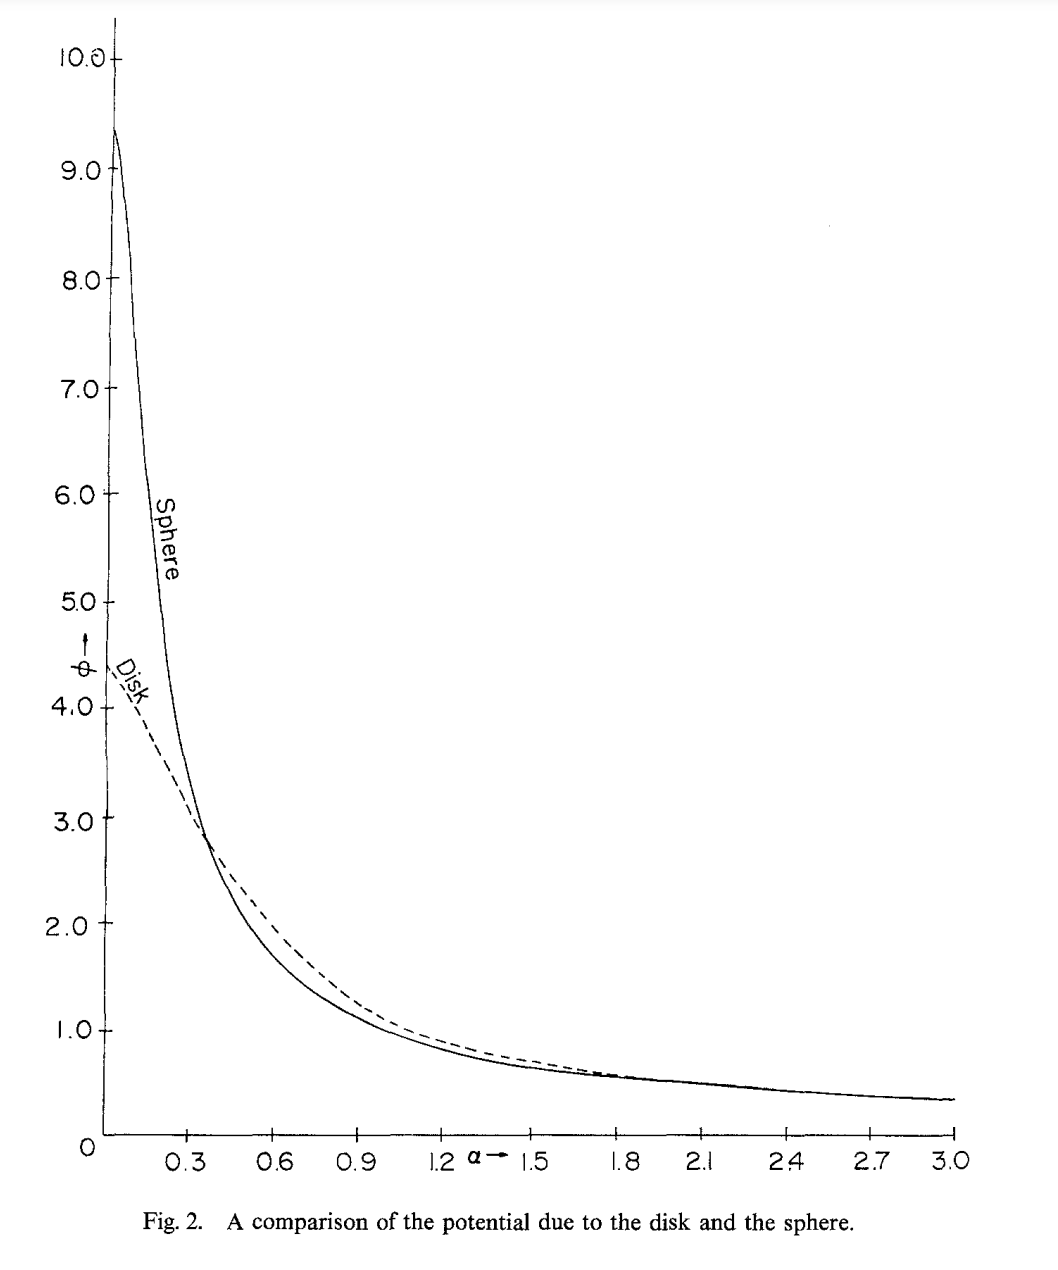
\includegraphics[width=\linewidth]{figures/Chatterjee_SphereDisk.png}
    \caption{ $\alpha = r/R$, for $R$ the radial extent of the stars \cite{Chatterjee}. Ask permission.}
    \label{fig:my_geom}
\end{figure}  
    
      
    

%%%%%%
%%%%%%%
%%%%%%
%%%%%%%
%%%%%%
%%%%%%% 
%%%%%%
%%%%%%
%%%%%%%  
%%%%%%
%%%%%%%  Do analysis on N7814 and N891
%%%Compare Fraternali y DM.
%%%%%%%
\section{Data \label{sec:data}}
 
 \subsection{SPARC Galaxies}
 We fit the Spitzer Photometry and Accurate Rotation Curves (SPARC) dataset  of  175 nearby galaxies with extended rotation curve data from atomic hydrogen (HI)  and H-$\alpha$ \cite{2016Lelli}. 
 HI provides the most reliable
 rotation curves because it is dynamically cold, traces circular orbits, and can be observed several effective radii past the stellar disk. 
 This sample of rotationally supported galaxies   spans the widest range of masses and morphologies currently available. 
 
These galaxies are  accompanied by model rotation curves representing   the  luminous mass components for each galaxy,  from   Spitzer Photometry in the 
   near infrared  at 3.6$\mu m$ interpreted in Poisson dynamics. 
   Near infrared  is  currently believed to be the best tracer of stellar mass   in population synthesis models (PSM) \cite{10.1093/mnras/sty3223}.  PSM, at this wavelength,   give mass-to-light ($\gamma_i$) ratios which are almost constant, independent of star formation history \cite{BelldYong,10.1093/mnras/sty3223}. Luminous mass rotation curves are reported in the SPARC database with all $\gamma_i=1$ in units of $M_{\odot} / L_{\odot}$   at 3.6$\mu m$. 
   PSM rely upon a complex  suite of  assumptions regarding galaxy evolution, metallicities and initial mass functions  \cite{BelldYong,10.1093/mnras/sty3223}, and are under-constrained  \cite{Conroy,Dutton_2005}.   
   
     Gas fractions $v_{gas}$ are calculated from surface density profiles of HI  with the formalism given in  \cite{1983MNRAS.203..735C} and scaled 
     a factor 1.33 to account for cosmological helium abundances.  Contributions from molecular gas are ignored   because CO data are not available for most SPARC galaxies. 
     Error on these velocities is estimated at $20\%$ \cite{2016Lelli}. 

   
   
     All terms in $\Phi(r)$ (Eq.~\ref{clocktime})  are    integrated from estimates of the baryonic mass as described in Sec.~\ref{sec:gravDets}, and as reported  in the      SPARC  library at \url{http://astroweb.cwru.edu/SPARC/}.    

 
   

  
%ASK STACY and compare to ours
 %Their final science sample is made of 153 galaxies.
 


%%%%%%
%%%%%%
%%%%%%%
\subsection{Milky Way}\label{MWselect}


The rotation curve fitting model presented here requires a static choice for the baryon distribution of the   Milky Way (MW). 
Mass-modeling of the MW is an under-constrained problem, due to     observing from       within  the disk  \cite{1991ARA&A..29..409F}.
 Beyond our position at 8 kpc, the data is very 
 noisy, see  Fig.~\ref{fig:mwSofue}.  
 
 
 We test the RCFM   using two different, static MW choices; 
   a hybrid model combined from  \citet{Xue}, 
  \citet{Sofue}, \cite{sofue2009unified}, and 
  a model from  \citet{McGaugh_2019}. The Sofue and Xue MW are derived from the same data and same model assumptions, but are combined for coverage of   $[0,20]$ kpc
  (\citet{Sofue})   and  $[20,60]$ kpc  (\citet{Xue}). 
  
   The  two Milky Way models vary in their underlying assumptions regarding structure and gravitational behavior of the Milky Way. For example, McGaugh \cite{McGaugh_2019} assumes a galactic bar at the center and thus does not include velocity data of the inner 5 kpc of the Milky Way.  In contrast, the Xue-Sofue MW is centrally condensed, and the peak velocity is   at around $94$ parsecs, versus that for  the McGaugh MW   at  approximately  $6.55$ Kpc   \cite{McGaugh_2019}. See Table~\ref{tab:MWcompare} for more information.
%Both MW models come from    deconvolving the   luminous mass of the stellar disk  from the rotation curve data  using either MOND or dark matter models. 
   
   
   

 
    
  
  
  
  \begin{table*}[]
      \centering
       \caption{Comparison of the two Milky Way models used in this paper}
      \label{tab:MWcompare}
       \begin{tabular}{|c|c|c|c|c|c|}
      \hline
        Milky Way Model & Photometry                        & Model dependence  & Rotation Curve data & scale radius bulge &$\gamma_{bulge}$\\
 \hline
Xue-Sofue     
&  2.2$ \mu m$
& NFW \cite{1996ApJ...462..563N}     
&SDSS DR6  \cite{Xue}       
& $Rb = 0.5$ kpc    
&$  7.1 M_\odot /L_\odot$  \\
  \hline
 McGaugh       
 & 3.6$\mu m$ 
 &MOND \cite{Milgrom}
 & CO data  \cite{2006ApJ...641..938L}                            
 &  N.A.  bar assumed
 & N.A. bar\\
         \hline
      \end{tabular}
     
  \end{table*}
  
  \begin{figure}
    \centering
    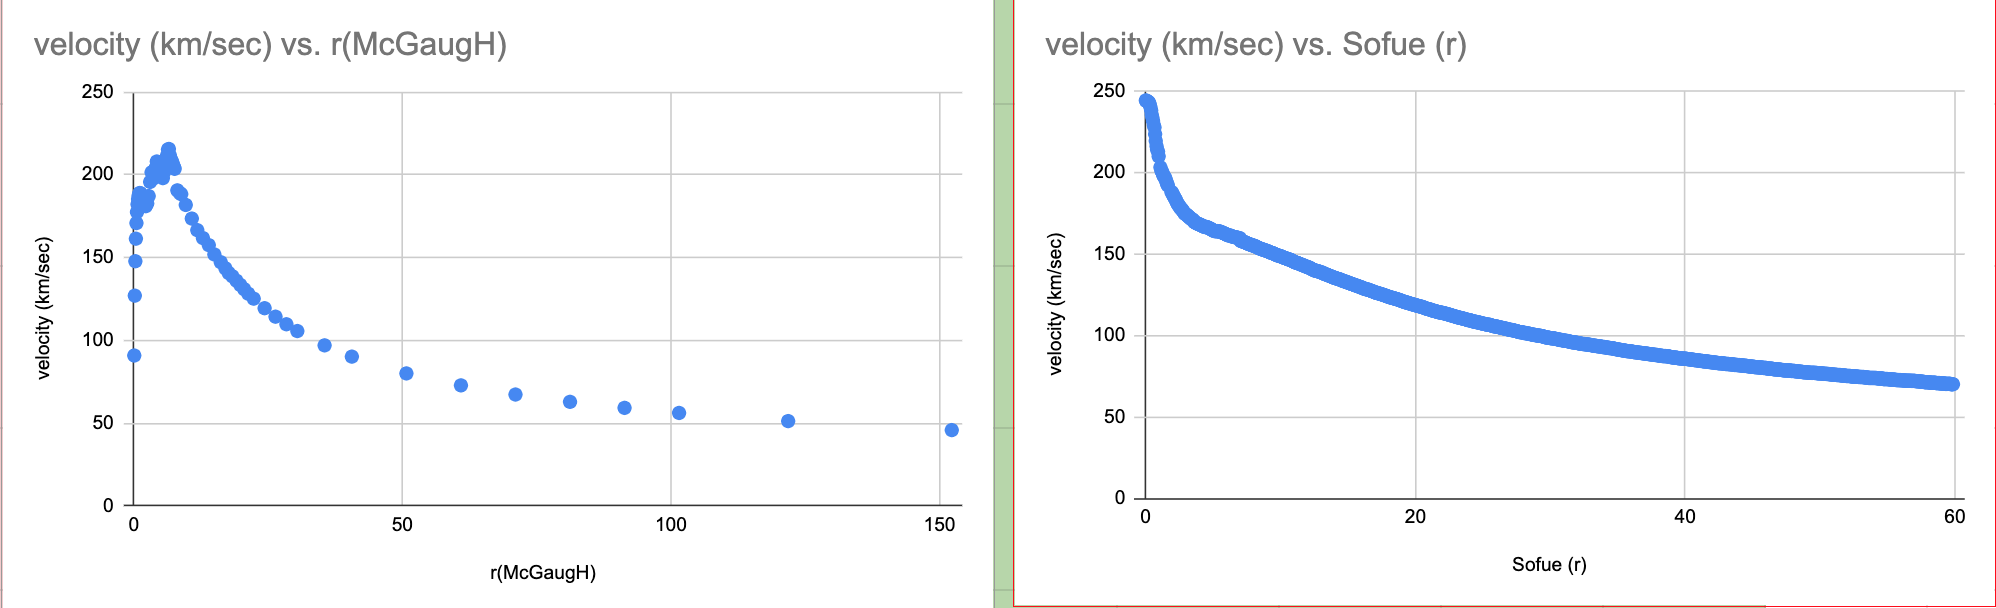
\includegraphics[width=\linewidth]{figures/MWXueSofueVMcGaugh.png}
    \caption{[REMAKE GRAPHS:  on same axes.] Milky Way rotation curves
   from Xue-Sofue and McGaugh \cite{sofue2009unified}, \cite{McGaugh_2019} }
    \label{fig:mwSofuevMcGaugh}
\end{figure}

 \begin{figure}
    \centering
    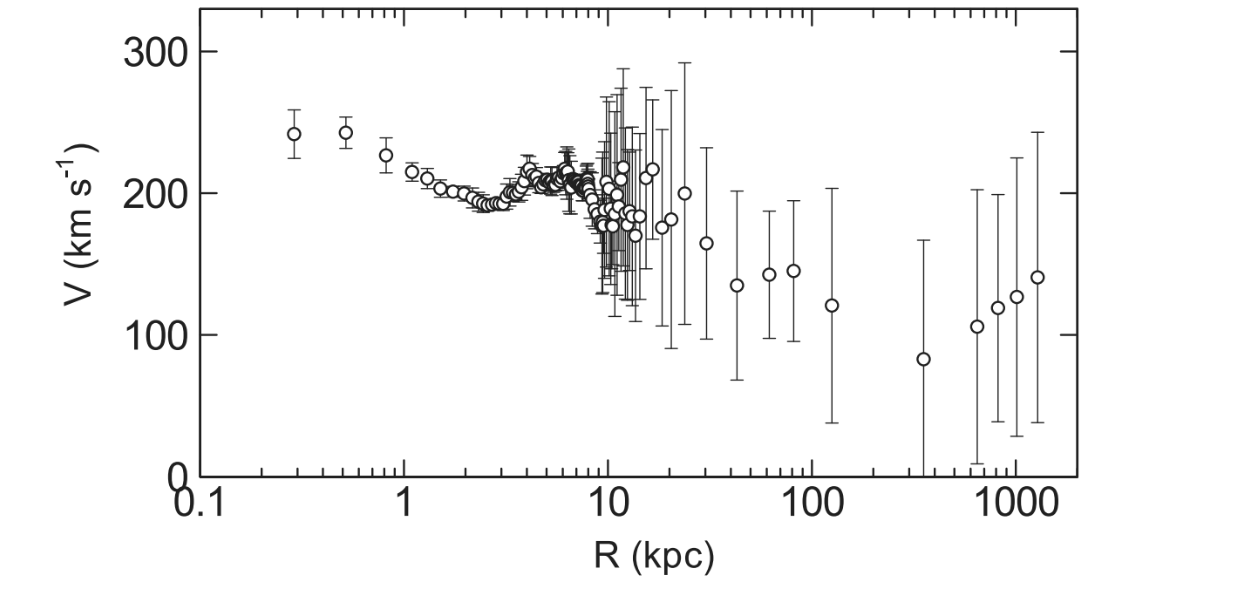
\includegraphics[width=\linewidth]{Sofue_MWtoLGData}
    \caption{ Milky Way rotation curve data from radio signals and SDSS CO star line shifts  \cite{Sof11}. Ask permission.}
    \label{fig:mwSofue}
\end{figure}

%Sofue: We included the circular velocities from an SDSS blue stars analysis by Xue et al. (2008; their model 1) by correcting for a systematic difference in the veloc-ities of about 20 km s1, due to our V0 = 200 km s1 instead of their 220 km s1.
%ugggh. have to look at the first two papers to see what assumptions they make. 
%We decomposed the newest rotation curve into a de Vaucouleurs bulge, an exponential disk, and an isothermal dark halo (Sofue et al. 2009).
%OBS METHOD: 
%An inner rotation curve was obtained by a terminal-velocity method applied to radio line observations
% An outer rotation curve was obtained by combining the CO star line velocities and the optical distances
%and by the HI disk-thickness method
%de Vaucouleurs bulge of mass Mb = 1.8 1010 Mˇ with a scale radius of Rb = 0.5 kpc, an exponential disk of mass Md = 71010Mˇ with a scale radius of Rd = 3.5 kpc,
%In the inner Galaxy at R .10 kpc, the rotation velocity is predominantly determined by the bulge and disk contributions, and R < 0.5 kpc it is almost determined by the bulge alone.


  
%   \begin{table*}[h!]
%      \centering
%      \begin{tabular}{|c|c|c|}
%      \hline
%        Author & Position of the Solar system   &  scalelength disk\\
%        \hline
%        Sofue \cite{sofue2009unified,10.1093/pasj/61.2.153,Sof11}   & 8 kpc &\\
%             \hline
%        McGaugh\cite{2021DDA....5240103M} & &\\
%         \hline
%        Klypin&&\\
 %        \hline
%        Enbang Li&&\\
%         \hline
%      \end{tabular}
%      \caption{MW}
%      \label{tab:my_label}
%  \end{table*}
  
 

 


 








\section{  Analysis and Results \label{sec:analysis}}
 
 

 
 
 


%{\color{blue}\emph{COMMENT MEAGAN: We'll want a better title, and this is basically a first draft.  Also, this probably isn't the right order to do things in. Maybe we should first address which galaxies we analyze, then the actual fitting, then interpreting $\alpha?$} }


\subsection{fitting procedure}



To fit galaxies in the SPARC sample,  the fitting procedure is as follows.   First,  a       Milky Way model must be chosen (see Sec.~\ref{MWselect})  and the data  read in as $v_{lum}(r)$ for a series of measurements in radii. The galactic potential is computed as per Eq.~\ref{eq:Newt2} by numerically integrating

\begin{equation}
\Phi(r) = \int_{inner}^{outer} dr \frac{ 
v(r)^2_{lum} 
}{r}.
\label{nowthen}
\end{equation}

Once the MW potential is calculated, it remains static for the rest of the fitting procedure.  

The data for the   galaxies being observed include several pieces of information: the rotation curve velocities $v_{obs}(r)$ from Doppler shifted spectra, the uncertainty on that measurement $v_{err}(r)$, and the components of the luminous mass interpreted as orbital velocities,  $v(r)_{bulge}$, $v(r)_{disk}$, and $v(r)_{gas}$. 
To calculate the baryonic potential for the galaxy in question, $v_{lum}(r)$ is first computed   as per Eq.~\ref{eq:zonte3}, for $\gamma_b=1$ and $\gamma_d=1$. The $\Phi_{gal}(r)$ associated with that galaxy   is then computed as in Eq.~\ref{nowthen}.

After the $\Phi(r)$ for the galaxy being studied and the Milky Way have been calculated,   the components must be compared at  matching values of $r$. To match radii, the $\Phi_{MW}(r)$ are calculated at  interpolated   radii as reported in the 
rotation curve data $v_{obs}(r)$ for the galaxy being observed. Any point with a radius larger than the largest radius in the Milky Way model is discarded.

The terms in the RCFM   can then be calculated  to produce the  $v_{rc}$ in Eq.~\ref{eq:zonteLCM}, which is  fitted to the  $v_{obs}$. 

 
%({\color{blue} I'm not sure we need to do all this algebra for them....??? }
%To calculate $v_1$ and $v_2$,   the terms $e^\zeta$ and $e^\eta$ are needed, which we rename for convenience. These are as defined in equations (REF) and (REF)

%\begin{equation}
%    \psi_{curve}(r) = e^\zeta = \sqrt{\frac{1 - %2\Phi_{gal}(r)}{1 - 2\Phi_{MW}(r)}}
%\end{equation}

%\begin{equation}
%    \psi_{flat}(r) = e^\eta = \sqrt{\frac{1 + %\beta_{gal}(r)}{1 - \beta_{gal}(r)}}
%\end{equation}

%Where

%\begin{equation}
%    \beta_{gal}(r) = \frac{v_{lum,gal}(r)}{c}
%\end{equation}

%Then the $v_1$ and $v_2$ terms are the respective hyperbolic functions.

%\begin{equation}
%    v_1(r) = \sinh(\eta) = \frac{\psi_{curve}^2(r) - 1}{2 \psi_{curve}(r)}
%\end{equation}

%\begin{equation}
%    v_2(r) = \cosh((\zeta + \eta)/2) = \frac{\psi_{curve}(r) \psi_{flat}(r) + 1}{
 %   2\sqrt{\psi_{curve}(r) \psi_{flat}(r)}}
%\end{equation}

The RCFM prediction is    assembled as in equation \ref{eq:zonteLCM}, to give a predicted $v_{rc}$ which is fitted to the rotation curve data $v_{obs}$. The fit is then minimized to find the  lowest   $\chi^2$,  using the {\tt scipy.optimize.curve\_fit} utility in Python.

The equations outlined in Section \ref{sec:dos} contain   free parameters that must be determined for each galaxy fit. The choice of the static Milky Way luminous mass profile is chosen before fitting,  the model's free parameter $\alpha$ ,  and the mass to light ratios for the  stellar bulge $\gamma_b$ and stellar disk $\gamma_d$ are determined during the fitting process by minimization of the $\chi^2$. 
The RCFM approach  has  the same number of free/constrained parameters as MOND and fewer than dark matter theories{\color{blue}\emph{(ASK STACY about this interpretation)} }.   What is more, the RCFM's free parameter $\alpha$ is well correlated to  observable photometric quantities (total luminosity and half light radius of the external galaxy).  
The mass-to-light parameters   are allowed to vary freely from an initial value of $1.0$, see Eq.~\ref{eq:zonte3}, and the $\alpha$ parameter     from an initial value of $\alpha = 0.01$. 

Reported gas fractions (HI scaled for Helium abundance) are fixed,  though addition of molecular gas could increase mass fractions in the inner kiloparsec of a galaxy   \cite{2004ApJ...609..652M}.





\subsection{Evaluating Goodness-of-fits}

There are two metrics by which rotation curve fits are judged. One, the reduced  $\chi^2$ values, and 
 two, the resulting mass-to-light ratios from   fits as compared to   PSM. 
The $\chi^{2}$ values for RCFM fits shown in Table~\ref{table:M2Light} and Table~\ref{tab:lobes} are remarkably low, providing confidence in the faithfulness of fits to rotation curve data.  
  While reported error    estimates on rotation curve velocities  have not been standardized across the field~\citep{Blok,Gent},     one can reliably   compare $\chi^{2}$ values  to the same rotation curve data. 
%The functional form of ${v_1}$ and ${v_2}$, the mapped velocities used in fits, had a major effect on $\chi^{2}$ of fits to the training set. The ${v_1}$ and ${v_2}$ functions chosen for use in our model resulted in the lowest $\chi^{2}$ and thus provided fits that described the data with the most accuracy according to that metric.
 In Table~\ref{tab:lobes}  the    average mass-to-light ratios for the entire sample are given for both RCFM and RAR fits ,  in comparison to expectations from PSM \citet{McGaugh2016RAR}.    {\color{teal} Ask Stacy about this interpretation: The $\gamma_d$ for the RCFM   are consistent with PSM within the stated error of $ 20\%$ \cite{2016Lelli} after scaling the average disk $\gamma_d$ down by a factor of 2 to compensate for the spherical integration procedure.   In Sec.~\ref{GeomSphere}, we discuss adjusting for use of  spherical approximation for the exponential disks for computational reasons.  }
  
    
    
    \begin{table}[h!]
        \centering
        \begin{tabular}{|c|c|c|c|c|}
        \hline
        &Model & $\gamma_d$ & $\gamma_b$& $\chi^2_{red}$ \\
        \hline
        \hline
           & PSM \cite{McGaugh2016RAR} & 0.5 &0.7&--- \\
            \hline
            \hline
         &   RAR	 &    0.64 &	0.73  & \\
         \hline
         &  RCFM   &  0.56 &	0.81&\\
           \hline\\ 
        \end{tabular}
        \caption{  {\color{teal}NOTE: rcfm disk scaled down by 2.}
          Average mass-to-light $\gamma_i$  ratios and reduced $\chi^2$  results from RAR and RCFM fits to the SPARC sample of 175 galaxies. The $\gamma_i$ are in units of  solar mass per solar luminosity $M_\odot/L_\odot$. }
        \label{tab:lobes}
    \end{table}
    
    
   \subsection{Comparing Milky Way Models} 
   
   
    The residuals of fits to the SPARC sample were used to compare different Milky Way models (see Sec.~\ref{MWselect}).  Histograms of residuals normalized by the error in velocity observations are shown in Fig.~\ref{fig:residual graphs}. 
     In all cases, residuals of model fits to observed velocity data followed a narrow distribution centered at zero with a range of +/-3 km/s, albeit with heavy tail features.  {\color{blue}Ask Stacy about this interpretation: The behavior of the residuals did not vary greatly between Milky Way models, suggesting that the fitting parameters in our model are robust with respect to differing Milky Way model assumptions.} 
    
    A Gaussian fit on residuals from fits using the McGaugh Milky Way model gave a mean of $-0.027$ km/s, standard deviation of $0.841$ km/s and a full-width half-maximum (FWHM) of $1.980$ km/s, whereas a Gaussian fit to the residuals from fits using the XueSofue Milky Way model gave a mean of $-0.012$ km/s, standard deviation of 0.819 km/s and a FWHM of  $1.928$ km/s. The small values associated with these quantities in both cases provide confidence that our fits match data closely.
    
    
\begin{figure*}[h]
     \centering
     \begin{subfigure}[b]{0.475\textwidth}
         \centering
         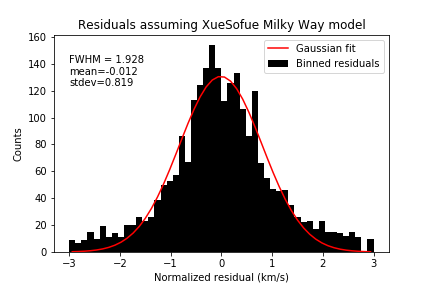
\includegraphics[width=.8\linewidth]{figures/ResidualHist_GaussFit_v1_sinh_v2_cosh_sparc128_newnorm_XueSofue.png}
         \label{fig:XueSofue residuals gaussian fit}
     \end{subfigure}
     \begin{subfigure}[b]{0.475\textwidth}
         \centering
         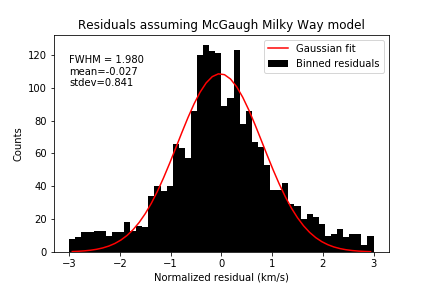
\includegraphics[width=.8\linewidth]{figures/ResidualHist_GaussFit_v1_sinh_v2_cosh_sparc128_newnorm_McGaugh.png}
         \label{fig:McGaugh residuals gaussian fit}
     \end{subfigure}
     \begin{subfigure}[b]{0.475\textwidth}
         \centering
         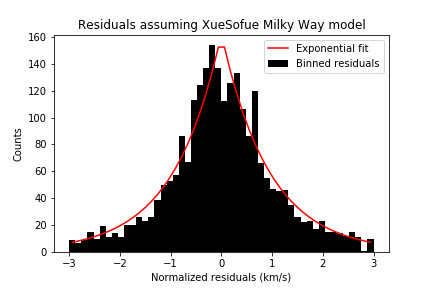
\includegraphics[width=.8\linewidth]{figures/ResidualHist_ExpFit_v1_sinh_v2_cosh_sparc128_newnorm_XueSofue.png}
         \label{fig:XueSofue residuals exponential fit}
     \end{subfigure}
     \begin{subfigure}[b]{0.475\textwidth}
         \centering
         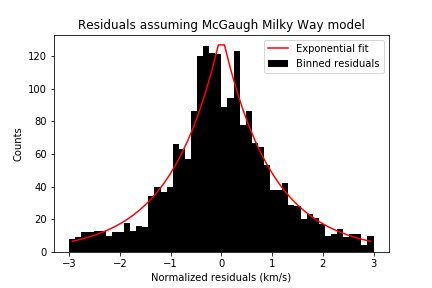
\includegraphics[width=.8\linewidth]{figures/ResidualHist_ExpFit_v1_sinh_v2_cosh_sparc128_newnorm_McGaugh}
         \label{fig:McGaugh residuals exponential fit}
     \end{subfigure}
        \caption{Normalized residuals from fits assuming either XueSofue of McGaugh Milky Way models, fitted to a Gaussian or exponential function. The full-width half-maximums, means, and standard deviations are shown for the Gaussian fits. The exponential fits capture peak and tails in residuals better than the Gaussian fits, suggesting non-Gaussian behavior in the error of velocity observations.}
        \label{fig:residual graphs}
\end{figure*}
Yet, the Gaussian fits did not quite capture the full peak and heavy tails in the residuals. This suggests that there may be non-Gaussian error in the observations of galaxy velocities. To address this, the residuals were also fit to an exponential function shown in Fig.~\ref{fig:residual graphs}. The exponential function captured both the peak and the heavy-tailed behavior of the distributions more faithfully.

% NGC 3198 \cite{1985ApJAlbada} studies this galaxy, which MOND has troubles with. This galaxy has   a thin exponential disk (de Vaucouleurs 1959),(Freeman 1970).  \cite{Toky} mentions that MOND fails to fit NGC 3109, which we fit exceedingly well ($\chi^2 = 0.32$).NGC 2841 is also a problem for MOND
%%%%%%
%%%%%%%%
%%%%%%
%%%%%%%
%%%%%%


 \subsection{ Model Comparisons - individual galaxies}
 \label{results:MtoL}
 
   In this section will  
   compare RCFM   results to those from MOND, the Radial-Acceleration-Relation and dark matter models. 
   McGaugh extended MOND to a new empirical model called the Radial-Acceleration-Relation (RAR)  which maintains the idea of a changing acceleration scale, but arranges the functional dependence in a new way. The RAR represents the  global acceleration relation as
   
\begin{equation}
    g_{obs}=\frac{g_{bar}}{1-e^{-(\sqrt{g_{bar}/g_\dagger})}}
    \label{Eq:RAR}
\end{equation}

for all  terms in $g_i$   the gradient of the potentials as in Eq.~\ref{zoochance1}, for 
$ g_{bar}  $ that for   the baryons,    $g_{obs} $  that of   the rotation curve data, and   $v_\dagger = 3700 km^2/ s^2 kpc$  is the changing acceleration scale.  

 
 
 
\subsubsection{NGC 2841}

NGC 2841 is a star dominated spiral galaxy, which   historically, has been regarded as a problematic case for MOND  \citet{Gent}.   RAR   finds a good  fit for this galaxy    after adjusting
the Cepheid   distance of $14.1$ Mpc,  by $1\sigma$,  to $15.5$ Mpc. The RCFM fit is accomplished at the Cepheid distance, 
and has a comparable reduced $\chi^2$ to RAR. The resulting $\gamma_d$   are also commensurate.   The fits are compared side-by-side in  Fig.~\ref{fig:CompareNGC2841}. 

 \begin{figure*}[ht] 
  \begin{subfigure}[b]{0.5\linewidth}
    \centering
    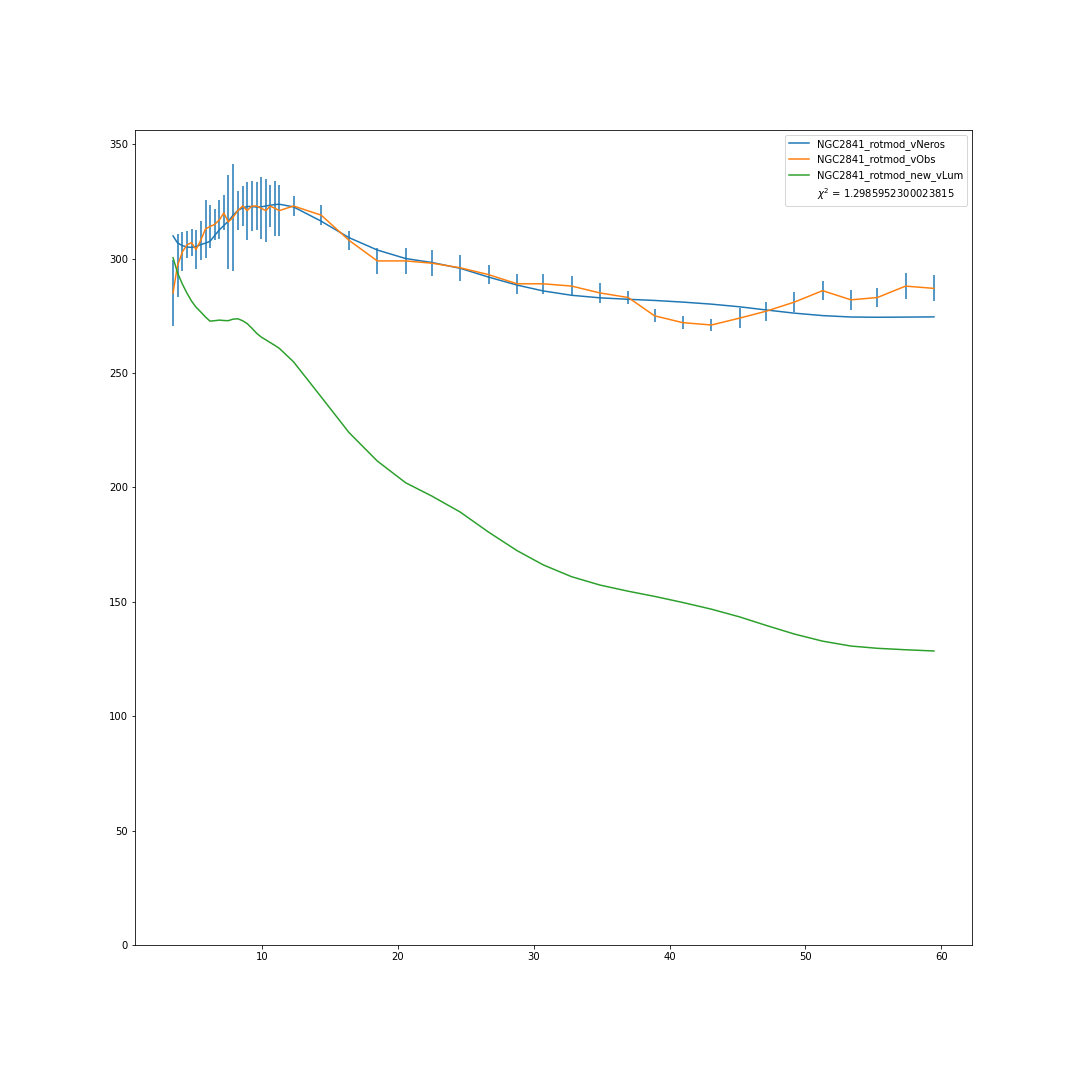
\includegraphics[width=0.95\linewidth]{figures/NGC2841_rotmod_XueSofue.png} 
    \caption{  RCFM fit is the blue line,  Green line is the Keplerian velocity due to  luminous mass estimates, and data points with error bars are the rotation curve data.
  Fitted at the 
    given Cepheid distance $14.1$ Mpc, with resulting mass-to-light ratios of  $\gamma_d = $    and $\gamma_b =1.11$, and  reduced  $\chi^2_\nu = 1.300$.  RUN AGAIN} 
    \label{fig:ngc2841RCFMfit} 
    \vspace{4ex}
  \end{subfigure}%% 
  \begin{subfigure}[b]{0.5\linewidth}
    \centering
    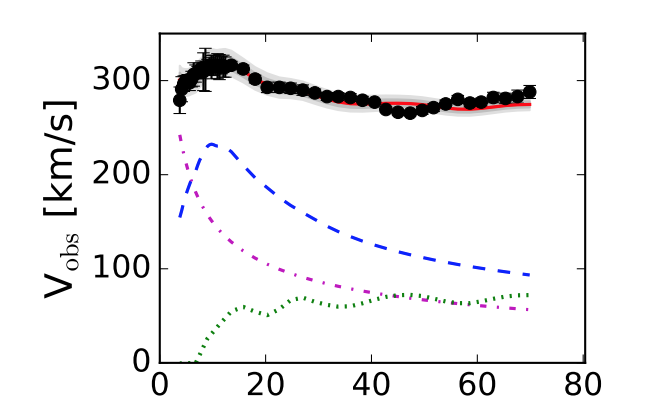
\includegraphics[width=0.95\linewidth]{figures/NGC2841_RarResults_Li2018}
    \caption{RAR fit is the red line, purple line is the bulge, blue is the disk, and green  is the gas \citet{Li_2018}.  ASK PERMISSION TO USE.   Distance parameter fit gives    $15.5\pm 0.7$ Mpc, $\gamma_d =0.81 $ and $\gamma_b =	0.93 $, and reduced $\chi^2_\nu = 1.515$. } 
    \label{fig:2841Li2018Rar} 
    \vspace{4ex}
  \end{subfigure} 
  \caption{Comparison fits to star dominated galaxy NGC2841 }
  \label{fig:CompareNGC2841} 
\end{figure*}

\subsubsection{IC 2574}

IC 2574 is  a gas dominated dwarf galaxy.
Figure \ref{fig:CompareIC2574} shows   fits to this galaxy from  the  RCFM in comparison to  NFW dark matter and RAR fits. 
 RAR finds a good fit to this galaxy    after adjusting
the  distance and inclination by $1-1.5 \sigma$, and their resulting disk mass-to-light 
$\gamma_d  = 0.07$ is  too low to be physical. 
This galaxy is also problematic for dark matter model fits, see Fig.~\ref{fig:Nav17} where the dark matter model significantly overestimates  the rotation curve to 10 kpc, \cite{2017MNRAS.471.1841N}.  
RCFM fit results for this galaxy give  $\gamma_d = 0.553$ , with no adjustment to the reported  tip of the red giant branch distance  of  $3.91$ Mpc. 




 
 \begin{figure*}[ht] 
  \begin{subfigure}[b]{0.5\linewidth}
    \centering
    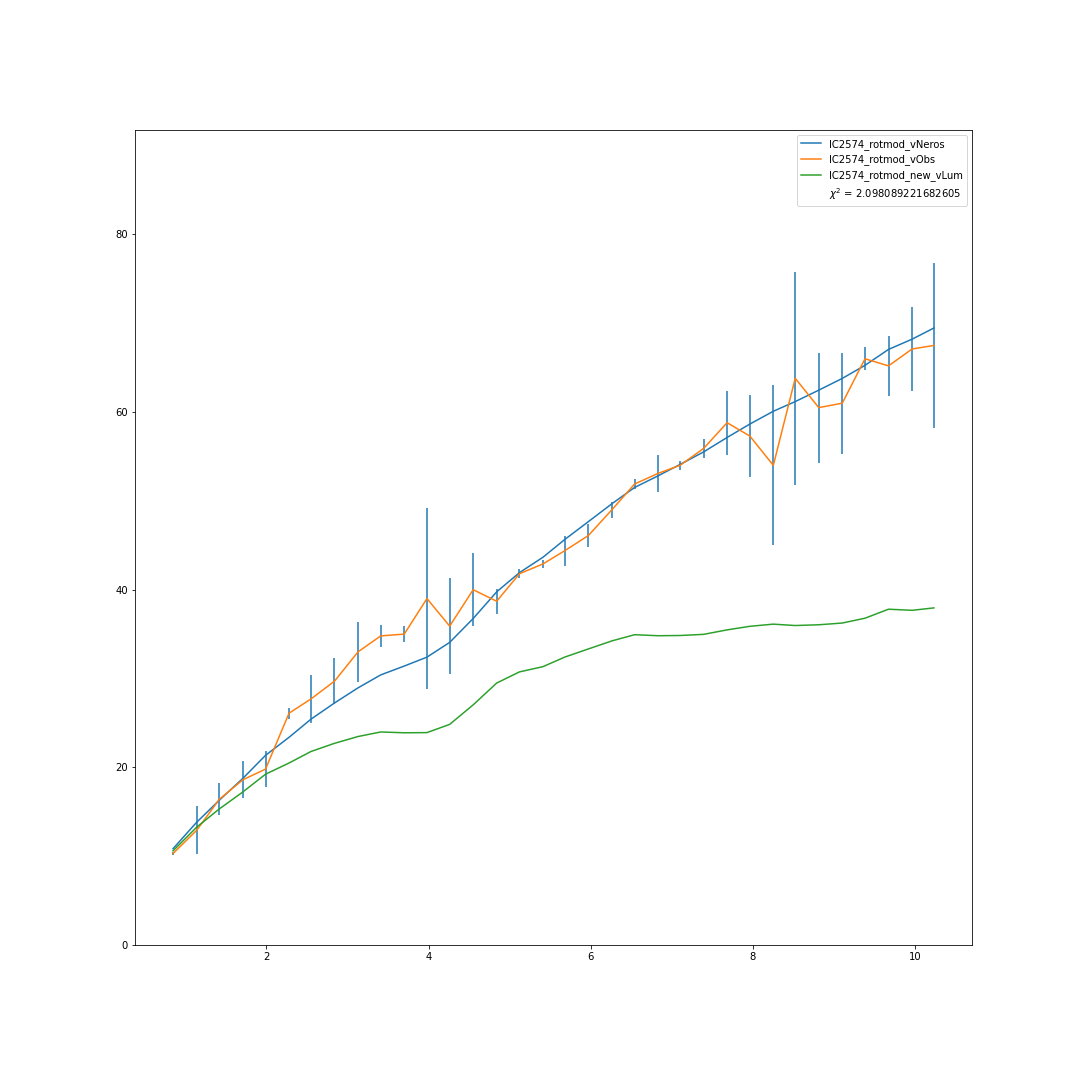
\includegraphics[width=0.95\linewidth]{figures/IC2574_rotmod_XueSofue.png} 
    \caption{  RCFM fit, 
    Fitted at the reported   distance $3.78 ± 0.19 $ Mpc from tip of the red giant branch, $\gamma_d = 1.105 $ (not scaled down by a factor of 1/2 yet), and reduced $\chi^2_\nu = 2.098  $.Lines are as in Fig.~\ref{fig:ngc2841RCFMfit}
    } 
    \label{fig:IC2574} 
    \vspace{4ex}
  \end{subfigure}%% 
  \begin{subfigure}[b]{0.5\linewidth}
    \centering
    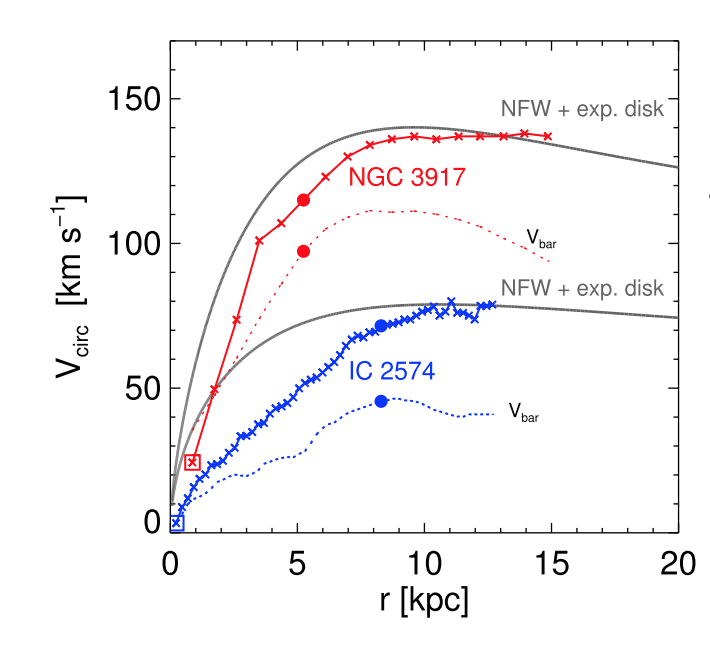
\includegraphics[width=0.95\linewidth]{figures/Navarro2017Fig3.png} 
    \caption{NFW dark matter fit, Figure from \cite{2017MNRAS.471.1841N}, ask permission. Parameter values not reported, but on inspection the dark matter model over predicts central rotation curve velocities.} 
    \label{fig:Nav17} 
    \vspace{4ex}
  \end{subfigure} 
    \begin{subfigure}[b]{0.5\linewidth}
    \centering
    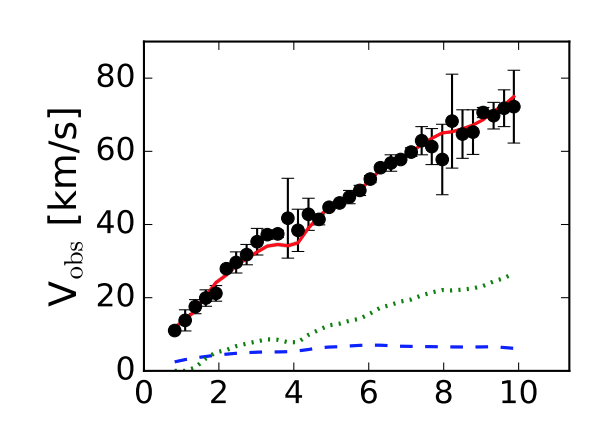
\includegraphics[width=0.95\linewidth]{figures/IC2574_Li.png} 
    \caption{  RAR fit (\cite{Li_2018})   ask permissions. Fit distance parameter gives a distance of $3.77 \pm 0.19$ Mpc, $\gamma_d =0.07 $, and reduced $\chi^2_\nu = 1.44$.Lines are as in Fig.~\ref{fig:2841Li2018Rar}} 
    \label{fig:Nav17} 
    \vspace{4ex}
  \end{subfigure} 
  \caption{ Comparison
fits to   gas dominated IC 2574  }
  \label{fig:CompareIC2574} 
\end{figure*}

\subsubsection{NGC 3198}

  NGC 3198 has historically been a problem  for MOND fits when the distance is a free parameter
\cite{Gent}, as the preferred distance for MOND fits is 2$\sigma$ smaller than that reported from  the most reliable distance indicator, Cepheid variable stars. RAR fits reproduce this distance preference, using a distance of
$ D = 10.4 \pm 0.4$ Mpc  \cite{Li_2018}. With this fit,  RAR gives a reduced
$\chi^2 = 2.057$, and $\gamma_d = 0.77 \pm 0.03$. The RCFM fit to  NGC 3198 at the Cepheid  distance  of 
$13.8$ Mpc, yields  a better reduced $\chi^2 = 1.676$, and mass-to-light ratios of  $\gamma_d = 0.439$.   See Fig.~\ref{fig1super}. 


 


    

   
   
 %TAM (NGC 3198, NGC 7793, and NGC 2976), we do not discuss NGC 7793 and NGC 2976 further, since the MOND fits present the same failures as the dark matter fits (in Newtonian dynamics), therefore we do not consider them as evidence against MOND. We just briefly note that in NGC 7793 the value of the inclination angle fitted by de Blok et al. (2008) is low and presents large variations in adjacent radii, which results in a poorly constrained rotation curve. In NGC 2976 the amplitude of the non-circular motions (Trachternach et al. 2008) is correlated with the amplitude of the fit residuals.
  
    \begin{figure*}[h!] 
    \begin{subfigure}[c]{0.5\linewidth}
    \centering
    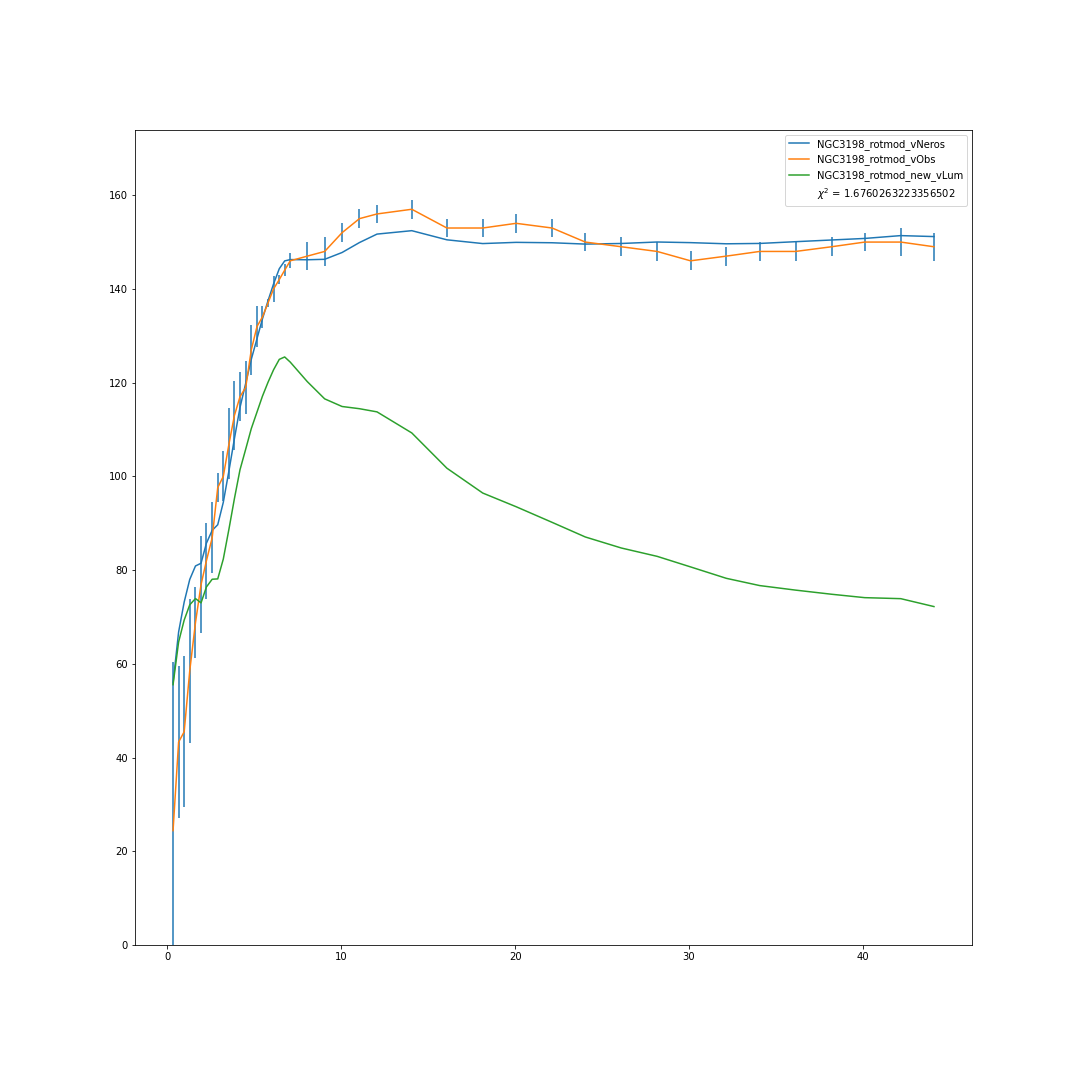
\includegraphics[width=0.95\linewidth]{figures/NGC3198_rotmod_XueSofue.png}
    \caption{RCFM fit blue line, at Cepheid based distance $13.8$Mpc,   luminous mass velocity  green line, reduced $\chi^2  =1.676$, $\gamma_d = 0.878$ (rotation curve data \cite{2016Lelli} }
    \label{fig:NGC3198RCFM} 
  \end{subfigure}%%
  \begin{subfigure}[c]{0.5\linewidth}
    \centering
    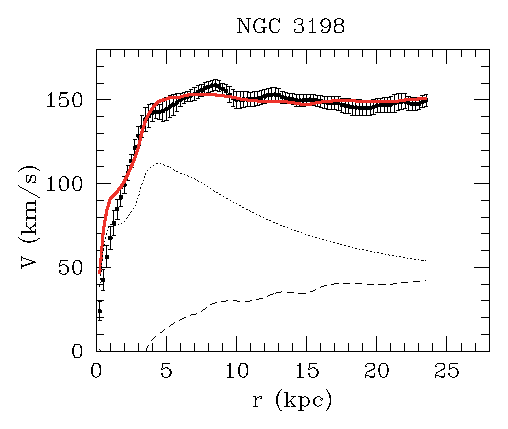
\includegraphics[width=0.95\linewidth]{figures/NGC3198_TAM_aa15283-10-fig7.eps} 
    \caption{ Image from \citet{Blok1}, ask permission.
    MOND fit red line  , at distance $8.6$ Mpc,    $\gamma_d =  1.01$ in the $3.6 \mu m$ band, $\chi^2=1.56$, $a_0 = 1.2 \times 10^{-8} cm/ s^2$ cm s-2. } 
    \label{fig:NGC3198MOND} 
  \end{subfigure}%%
  \caption{ Rotation Curve Fits   NGC 3198 }
  \label{fig1super} 
\end{figure*}


    \subsubsection{Comparison NGC 7814 and NGC 891}
  
 These two galaxies present an interesting conundrum for both dark matter and MOND models, because they are both presented edge-on, have 'essentially identical rotation curves'', and yet,  are extreme opposites in their morphology,  with NGC 7814 being bulge dominated and NGC 891 almost entirely a disk galaxy. 
 \citet{Frat1} asks, are these rotation curves are actually that identical?
 
 %% remove first point on N891_RotMod , Frat data, and Frat says is from noncircular motions
 
 
 In the context of the RCFM  paradigm, the two rotation are  very similar in magnitude,  but   differ markedly in the inflection  at large radii. 
 NGC 7814 inflects up, and  NGC 891 inflects down.
 In the RCFM paradigm, the inflection of rotation curves indicates   the total galaxy mass in baryons with respect to   the Milky Way.  
 
 However, the RCFM  
fits to these galaxies are successful, see Figures.\ref{fitCompare7814_891}). 
RCFM fits are to the same rotation curve data from   \cite{Frat}, and  use the baryon models reported from the SPARC database \cite{2016Lelli}. Since both of these galaxies are presented edge-on, they present a challenge to surface photometry, and so we demonstrate how the RCFM can constrain luminous mass modeling.
 
 
 
 \begin{figure*}
\centering
\begin{minipage}{.5\textwidth}
  \centering
  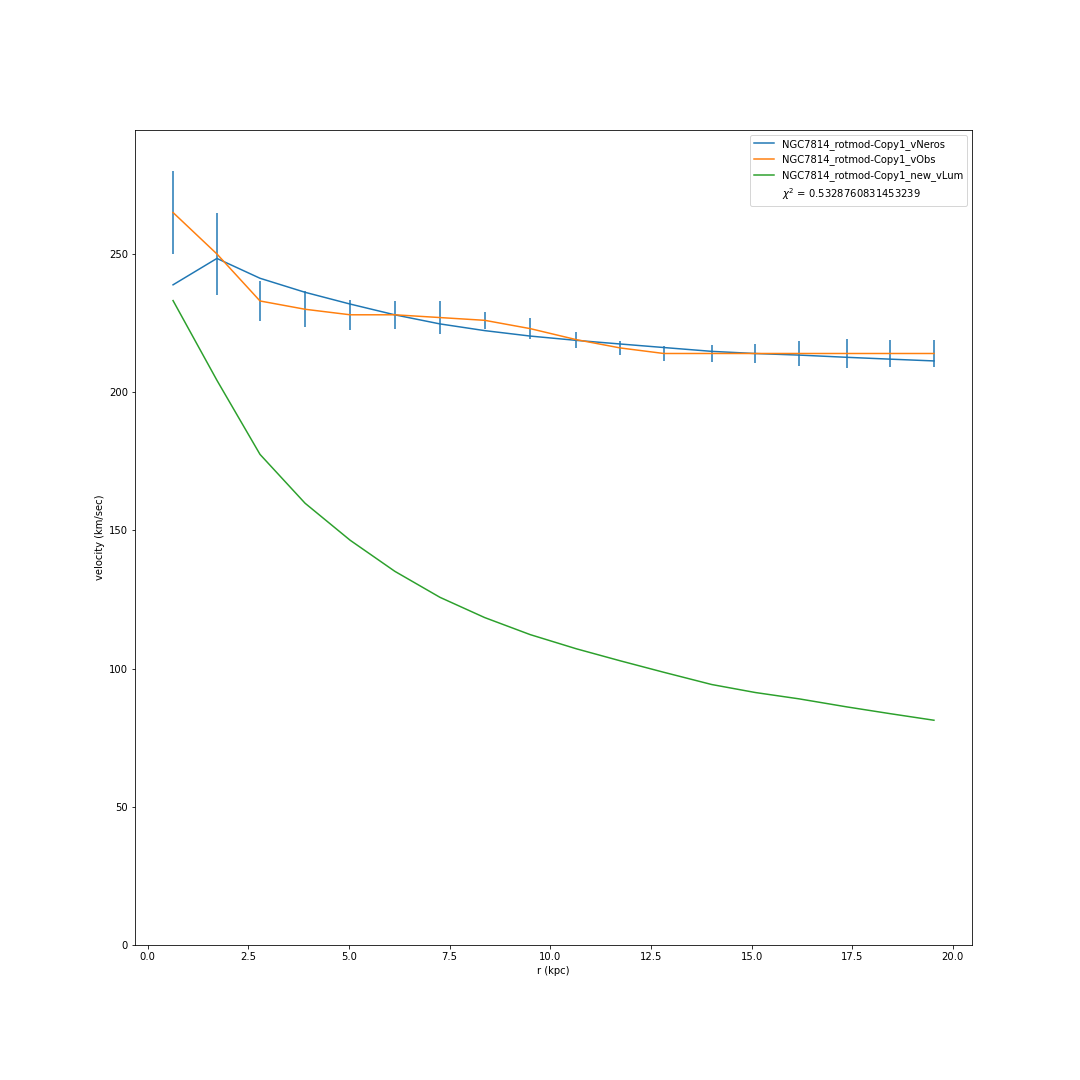
\includegraphics[width=.95\linewidth]{figures/NGC7814_rotmod-Copy1_XueSofue.png}
  \captionof{figure}{ NGC 7814, RCFM fit to SPARC\cite{2016Lelli}. Bulge dominated.}
  \label{fig:n7814sparc}
\end{minipage}%
\begin{minipage}{.5\textwidth}
  \centering
  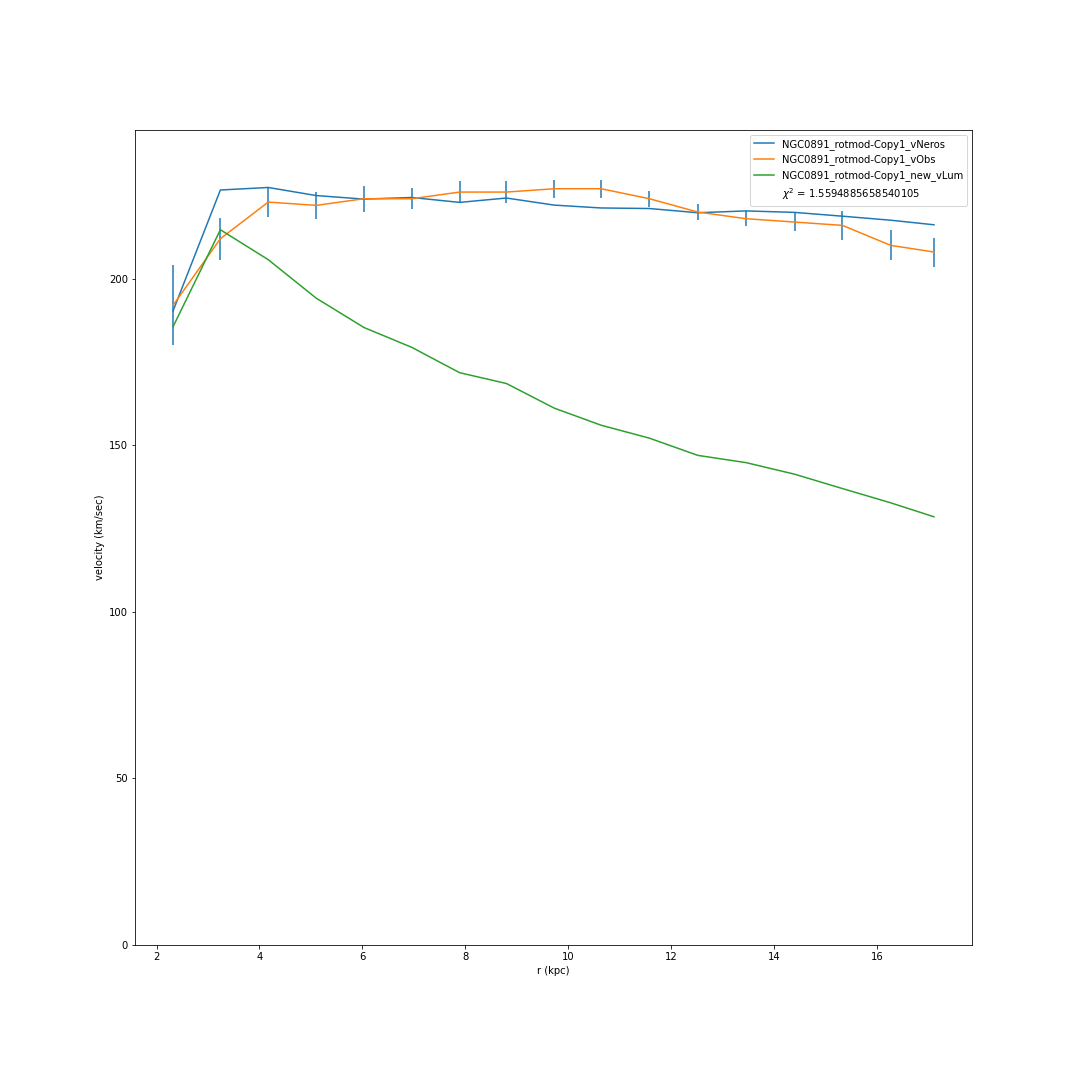
\includegraphics[width=.95\linewidth]{figures/NGC0891_rotmod-Copy1_XueSofue.png}
  \captionof{figure}{  NGC 891, RCFM fit to  SPARC\cite{2016Lelli},   Disk dominated }
  \label{fig:test1}
\end{minipage}
 \caption{Comparison of fits for NGC 7814 and NGC 891. Both edge-on galaxies with similar total light, but very different distributions of that light.     RCFM rotation curve fits (blue line), points with error bars are the rotation curve data, and the input baryonic mass models is  the green lines. {\color{blue}( (UPDATE FIGURES) } }\label{fitCompare7814_891}
\end{figure*}
 
 
 
 
  

\subsection{Free parameter functional form }\label{FreeCorrel}

  To test a guess at a functional form  for the  model's free parameter $\alpha$,  based on photometric quantities, we   select a subset of galaxies with the most reliable distances and rotation curve data. 
  The selection  criteria are \cite{2016Lelli}:  
  \begin{enumerate}
      \item photometry interpreted with most reliable  distance methods    (tip of the red giant branch, and Cepheid variable stars,  with errors in distance on the order of $5\% - 10\%$), rejecting all other galaxies. \\
      \item  inclination angle on the sky  in the range  $[15^o, 80^o]$, rejecting galaxies with an inclination  greater than $80^o$ as impossible to constrain the surface brightness profile, and those at inclinations less than $15^o$ as being impossible to  report line of sight Doppler shifts accurately.\\
      \item  \citet{2016Lelli}   report a quality factor for each galaxy in the SPARC database, assigning  $Q=3$ to galaxies not suited to dynamical studies due to     asymmetries,  non-circular motions, and/or offsets between stars and gas. Galaxies with Q = 3 are rejected from our subset.
%not suited for detailed dynamical studies:
  \end{enumerate}
    By this process, we select a subset of 36 galaxies as reported in Table~\ref{tab:Tset}. 


 We then plot the  $\alpha$   parameter  space versus the ratio of  photometric quantities,  
  
\begin{equation}
    L_{total}/R_{eff}, 
\end{equation}
 
 for  $L_{total}$    the  total luminosity of the galaxy as measured  at a wavelength of $3.6 \mu m$,  assuming a solar
absolute magnitude of 3.24 at $3.6 \mu m$ \cite{oh2008high}, and the effective radius $R_{eff}$    the length encompassing half of the total luminosity \cite{2016Lelli}. 
 The resulting distribution    (Fig.~\ref{alpha2}) is  well fitted by the function 
 
    
\begin{equation}
    \alpha =  
    53.8 (L_{total}/R_{eff})^{-1.06}
       \label{FreeParamFix}
\end{equation}

at a confidence level of $83\%$.
{\color{blue}(UPDATED From Master RCFM 2.8.23)}
  
 \begin{figure*}
%\scalebox{0.5}%
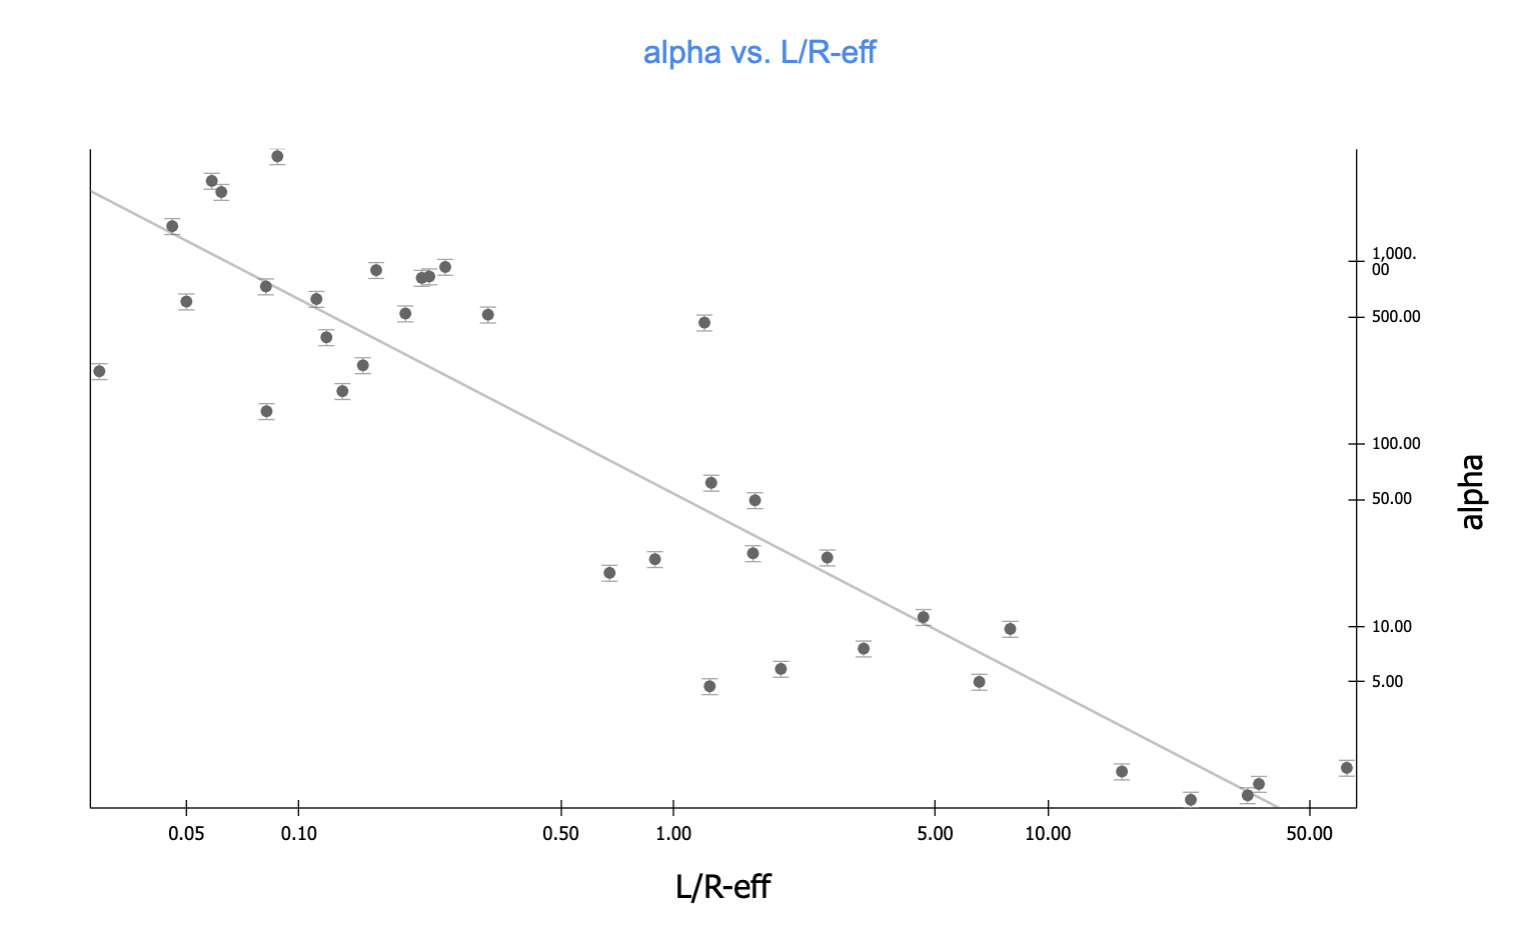
\includegraphics[width=\linewidth]{figures/alphavL_Reff2_8_23.png} 
\caption{  Training Set (Distances from Cepheids or Tip of the Red Giant Branch )  $L$, the  photometric parameter, is  in units of $10^9$ solar  $L_\odot$,  and the  photometric parameter $R_{eff}$ is  in kpc. List of galaxies see  Table~\ref{tab:Tset}.  {\color{blue}(updated. From GitMaster RCFM 2.8.23), Need to make prettier.  Errors not real, but could use those reported on SPARC for LUM}.  }
\label{alpha2}
\end{figure*}  
 
In the development of the RCFM, all quantities in $\kappa v_1 v_2$ are ratios between  the Milky Way and the galaxy being observed. If we extend that to the interpretation of the free parameter, then 
the functional form in Eq.~\ref{FreeParamFix}   suggests a ratio with the same quantity for the Milky Way. {\color{blue} Ask Stacy: estimates of $L_{tot}$ for the MW range from 200 billion M-sol, to 20 billion - the first number makes sense for this number (the quantity for the Milky Way  $42.94 =(L_{total}/R_{eff})_{mw} $, but if it's 20, and half-light radius is around 4 or 5, then this works}. 
  

%{\color{blue}RICH, The phrasing sounds extremely strange/confusing to me: "We might assume that alpha is a ratio of the same quantity for the Milky Way ..." What is that supposed to mean? That it's a possible higher order fitting function? \color{teal} I'm not sure if it's a higher order fitting function or if we even want to try to constrain fits using this functional interpretation, but it does make our model a zero param model. Then again, we already have at least one fewer free parameters than MOND or Dark Matter, so it maybe doesn't matter. }
 
  %%NOTE:  Details on SPARC Mass models. 
  %%%%%%SPARC uses hybrid rotation curves on 56 galaxies, combining H-alpha  (inner) with HI (outer)
 %Face-on gals in SPARC."We assign a quality flag (Q) to each rotation curve using the following scheme: Q = 1 for galaxies with high-quality H I data or hybrid Hα/H I rotation curves (99 objects); Q = 2 for
%galaxies with minor asymmetries and/or H I data of lower
%quality (64 objects); Q = 3 for galaxies with major asymmetries, strong noncircular motions, and/or offsets between H I
%nd stellar distributions (12 objects). Galaxies with Q = 3 are%
%not suited for detailed dynamical studies: we build mass models
%for completeness but do not consider them in our analysis.
 


 



 
 \section{  Conclusions \label{sec:conclu}  }
 




  
The RCFM can be seen  to reproduce the fitting successes of MOND and dark matter models,   on as  sample of   175  well studied galaxies\cite{2016Lelli},   but  without modifying physics.  This is accomplished by transitioning the idea of MOND's changing acceleration scale \cite{McGaugh2016RAR,2022A&A...664A..40M} to the concept of changing relative curvatures between galaxy frames. 
Previous consideration of frame-dependency in this problem was obviated by Galilean subtraction of redshifts at the limit of the rotation curve data\cite{Wald}.
 
Compare number of free parameters:    {\color{blue}(  MOND: distance and acceleration scale )}  {\color{blue}(  DM: variously 2-4??)} {\color{blue}( RCFM: MW and $\alpha = L/r_{eff} $)}.
Also, in the RCFM all    parameters can be constrained by photometry  (baryonic mass of the Milky Way and
$\alpha \prop L/R_{eff}$), and so this provides a unique opportunity to constrain population synthesis model interpretations of photometric measurements through the orthogonal observation of  Doppler shifted spectra. 
  
 
Since the  RCFM  proposes that dark matter is due to a frame-dependency, it is falsifiable by a well-determined rotation curve observation for the Milky Way,  at radii past our position at $\approx 8 kpc$.  As can be seen in Fig.~\ref{fig:mwSofue}, the rotation curve of the Milky Way  is ambiguous  past  $8$kpc  in 
  the galactic disk. Upcoming large surveys of the Milky Way  could accomplish this  \cite{Ivezić_2019,2022ApJS..259...35A,2010ApJ...716....1B,de_Blok_2010}. 

 
 
  
  
 %In example, the James Webb Space Telescope may have already falsified dark matter driven galaxy formation \cite{2022arXiv221014915H}.
   

  \section[]{Acknowledgments}
 This work is dedicated to Emmett Till, with   gratitude to the first nations peoples on whose unceded lands this was written on, including but not limited to  the Coast Salish bands of the Puget Sound, 
 the Cheyenne, Arapaho and Ute  Peoples of Colorado, and the Algonquian Peoples of Massachusetts. 
  The authors would like to thank    V.\,P.\,  Nair,   R.\, Walterbos, S.\ McGaugh,  A.\, Klypin, K. Bender, C. Beetle,     T.\, Boyer, and M. Juric.   \\
  
 
% QUESTION FOR GROUP: how is our model predictive, more so than MOND, since we both do well on fitting galaxies. The Milky Way. We get a large enough sample of galaxies with certain distances and good photometry (SPARC) and run against a two MW. 
%ANSWER FOR GROUP: Our is twice as good on average chisquare value across the whole sample, has same number of free parameters as MOND, (our our MW and alpha) (MOND's are acceleration scale and distance), and we about the same for the mass-to-light ratios as compared to the populations synthesis models. The key science difference is our reproduces rotation curves of very well studied galaxies with super reliable distance indicator (Cepheid variable stars) at the correct distance and MOND has to put them at distances that are up to 2sigma different. ALso, MOND requires modication of Einsteins' gravity, which is super well tested at least locally, and our doesnt'. So, for my money, we win. SNC.

%%%%%%%
 

\begin{figure*}
\centering
\begin{minipage}{.5\textwidth}
  \centering
  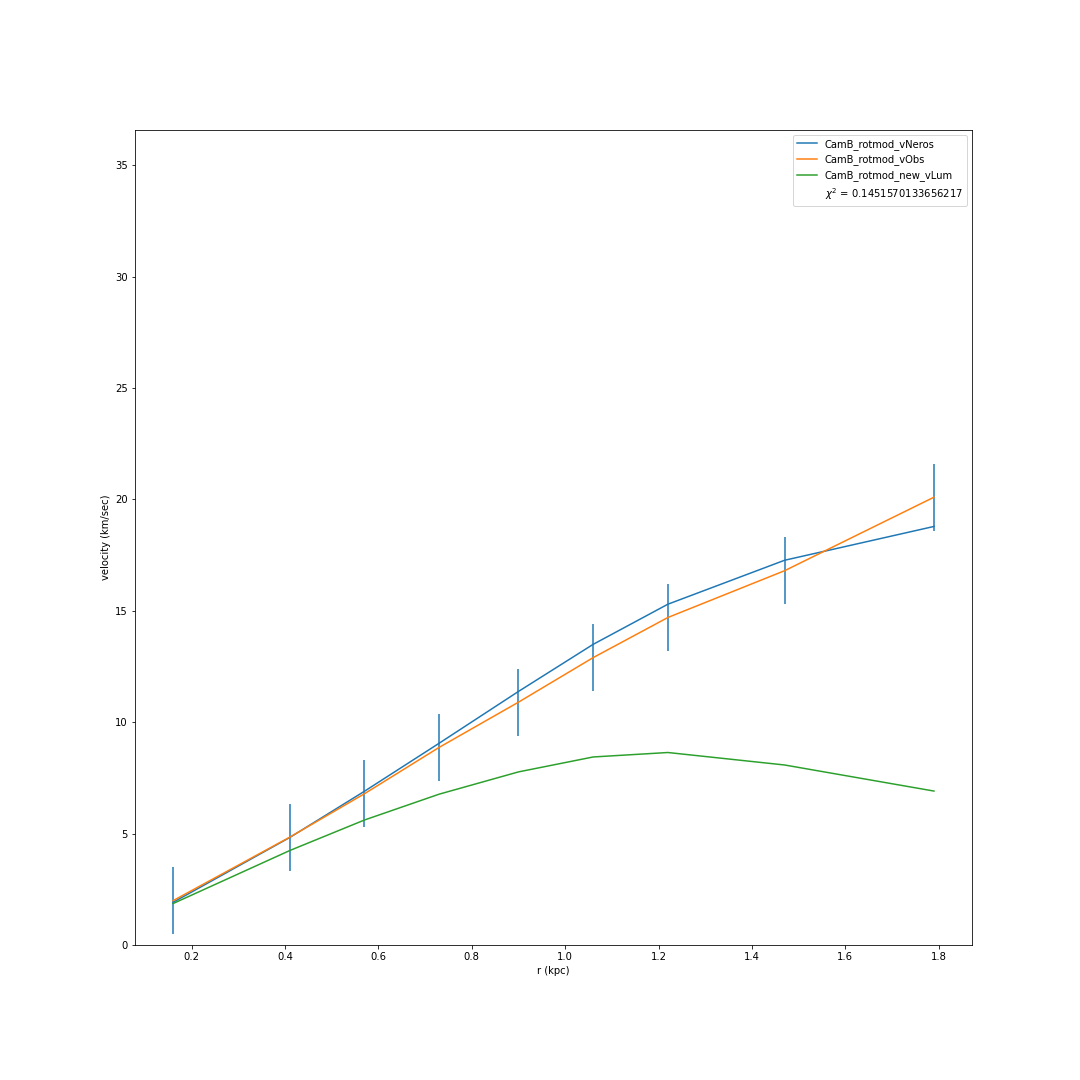
\includegraphics[width=.95\linewidth]{figures/CamB_rotmod_XueSofue.png}
  \captionof{figure}{CamB : SPARC\cite{2016Lelli}}
  \label{fig:test1}
\end{minipage}%
\begin{minipage}{.5\textwidth}
  \centering
  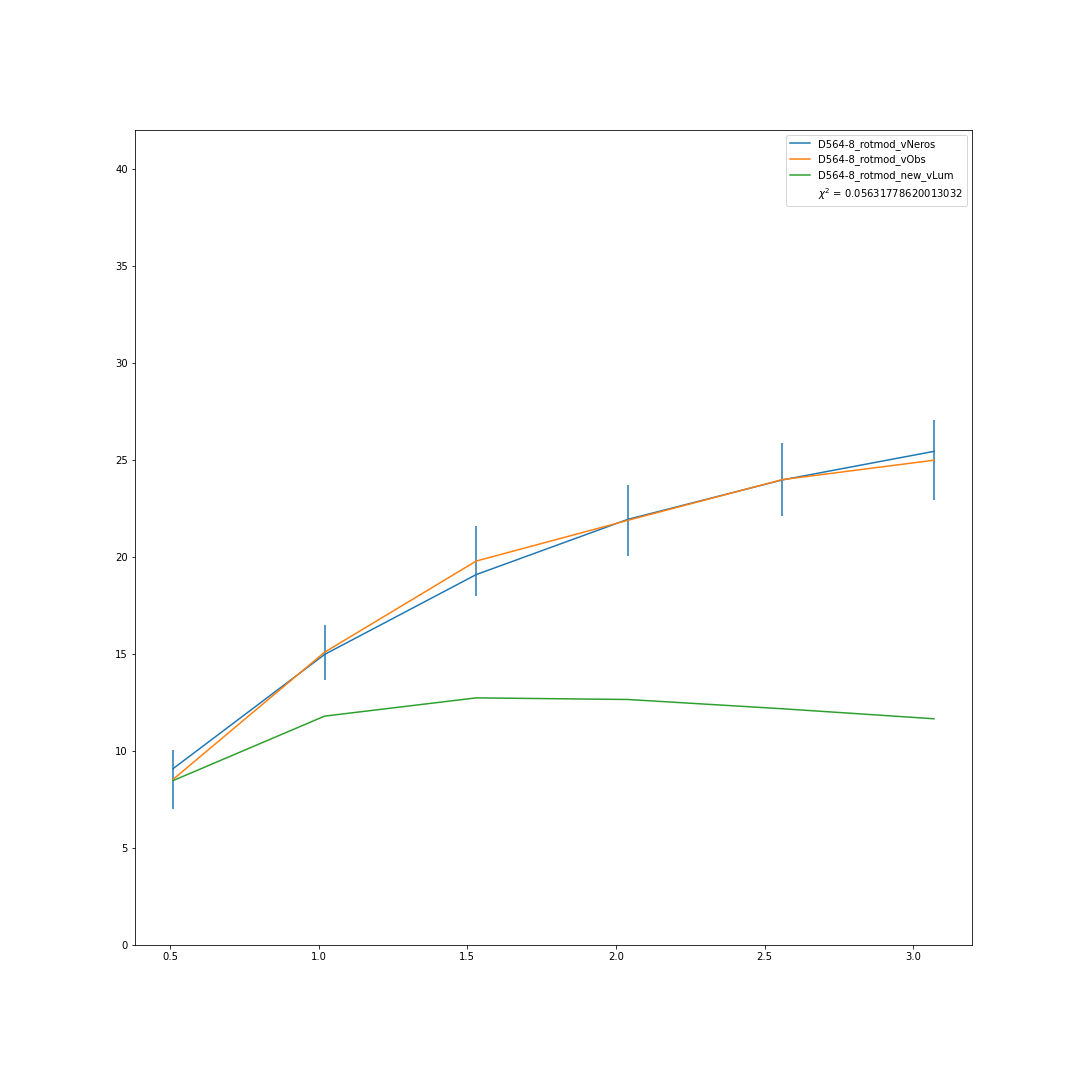
\includegraphics[width=.95\linewidth]{figures/D564-8_rotmod_XueSofue.png}
  \captionof{figure}{D564-8 : SPARC\cite{2016Lelli}}
  \label{fig:test2}
\end{minipage}
\begin{minipage}{.5\textwidth}
  \centering
  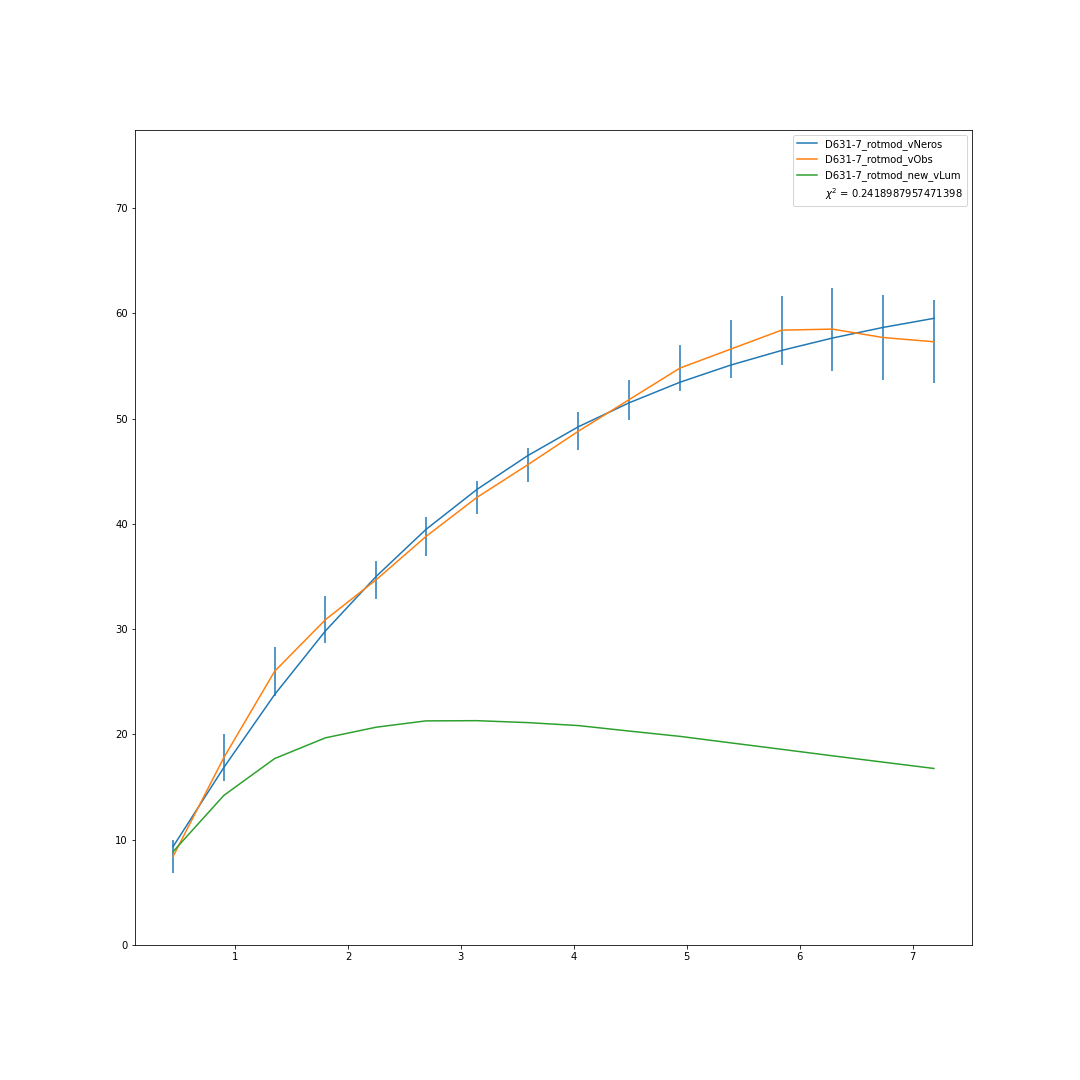
\includegraphics[width=.95\linewidth]{figures/D631-7_rotmod_XueSofue.png}
  \captionof{figure}{D631-7  SPARC\cite{2016Lelli}}
  \label{fig:test1}
\end{minipage}%
\begin{minipage}{.5\textwidth}
  \centering
  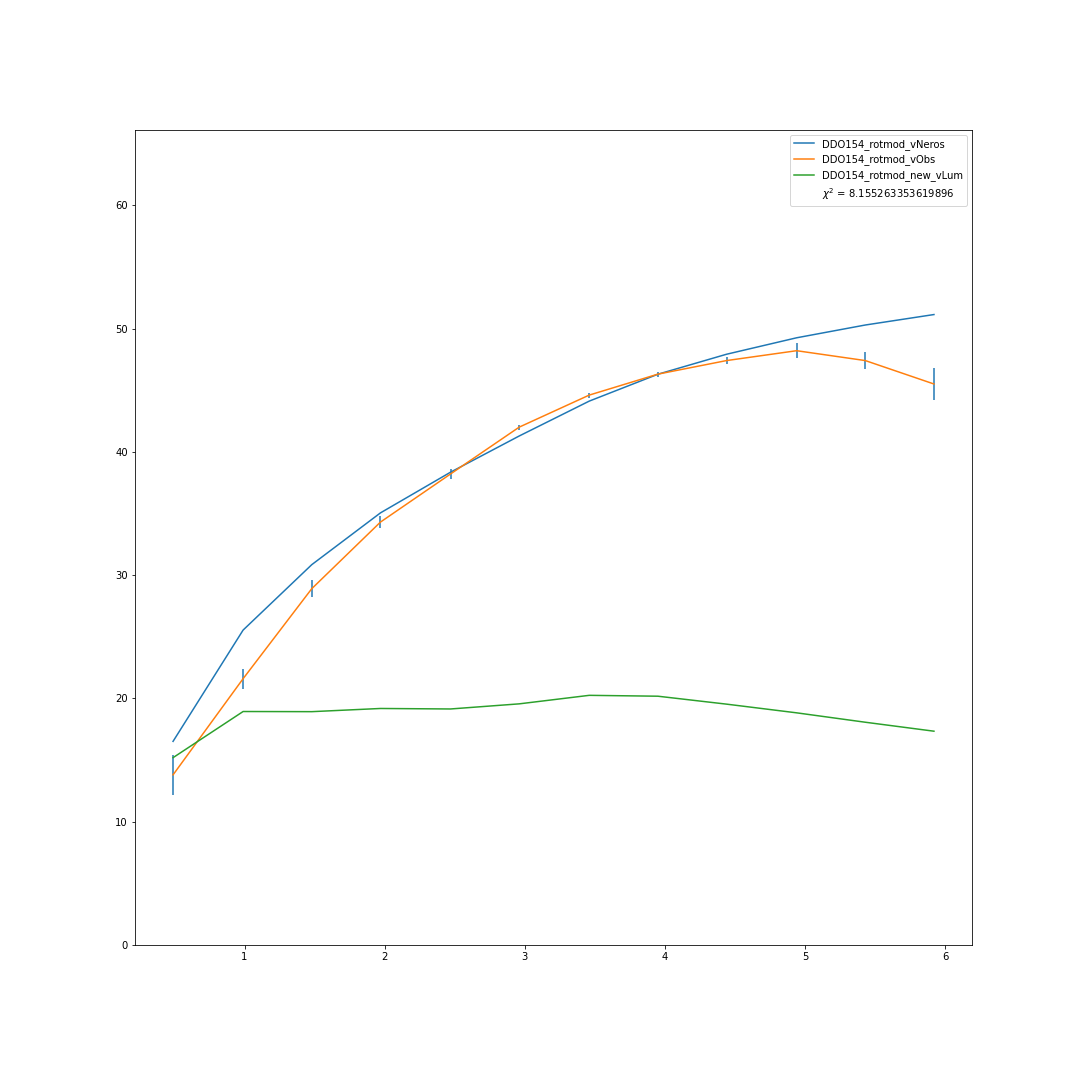
\includegraphics[width=.95\linewidth]{figures/DDO154_rotmod_XueSofue.png}
  \captionof{figure}{DD00154 : SPARC\cite{2016Lelli}}
  \label{fig:test1}
\end{minipage}
 \caption{Examples of range of gas dominated, dwarf galaxies, their RCFM rotation curve fits (blue line), points with error bars are the rotation curve data, and the input baryonic mass models is  the green lines. (MARCUS PAZ : NOTE: remove orange lines, fit through data distracts from our fit)  }
\end{figure*}
 
            
\begin{figure*}
\centering
\begin{minipage}{.5\textwidth}
  \centering
  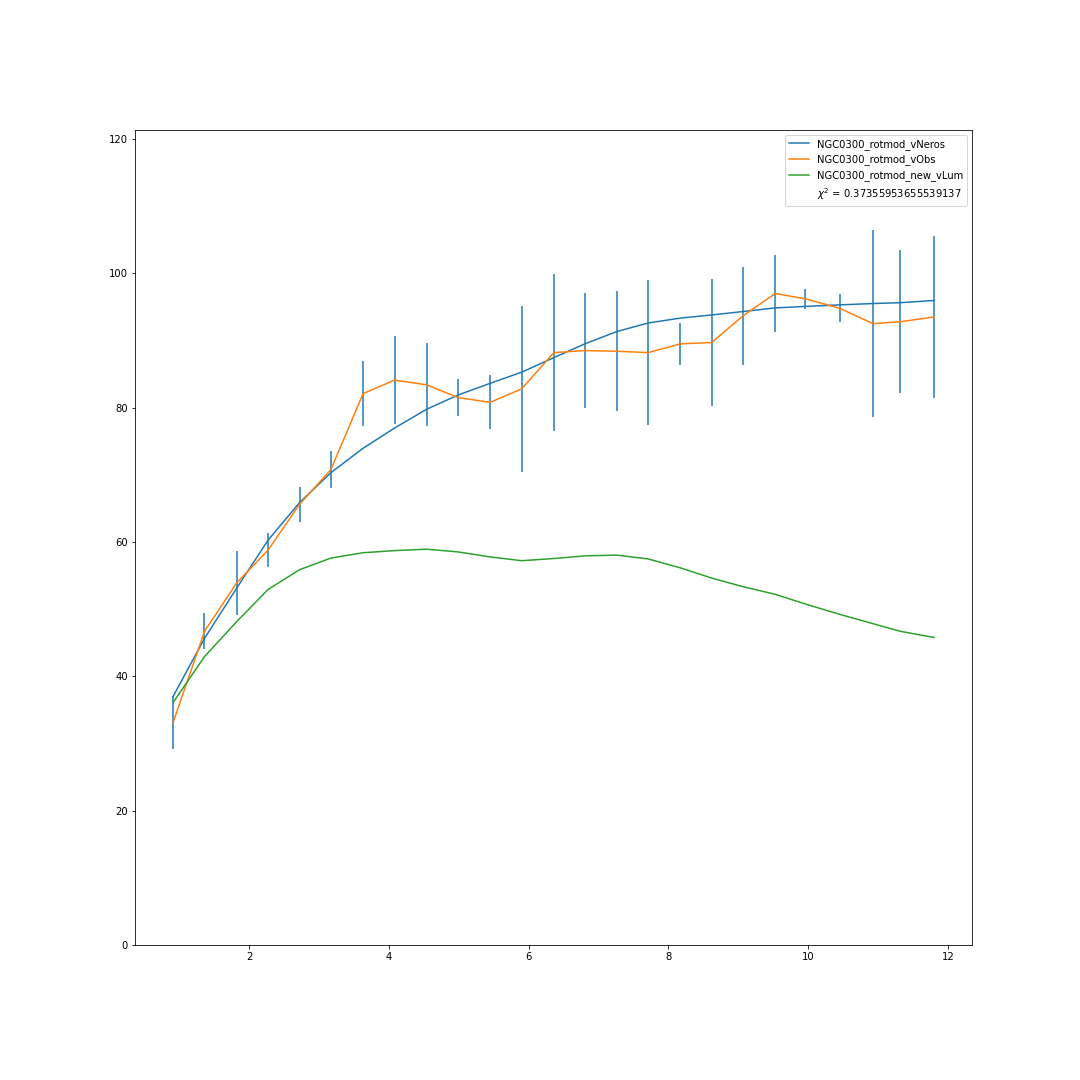
\includegraphics[width=.95\linewidth]{figures/NGC0300_rotmod_XueSofue.png}
  \captionof{figure}{ NGC0300 SPARC\cite{2016Lelli}}
  \label{fig:test1}
\end{minipage}%
\begin{minipage}{.5\textwidth}
  \centering
  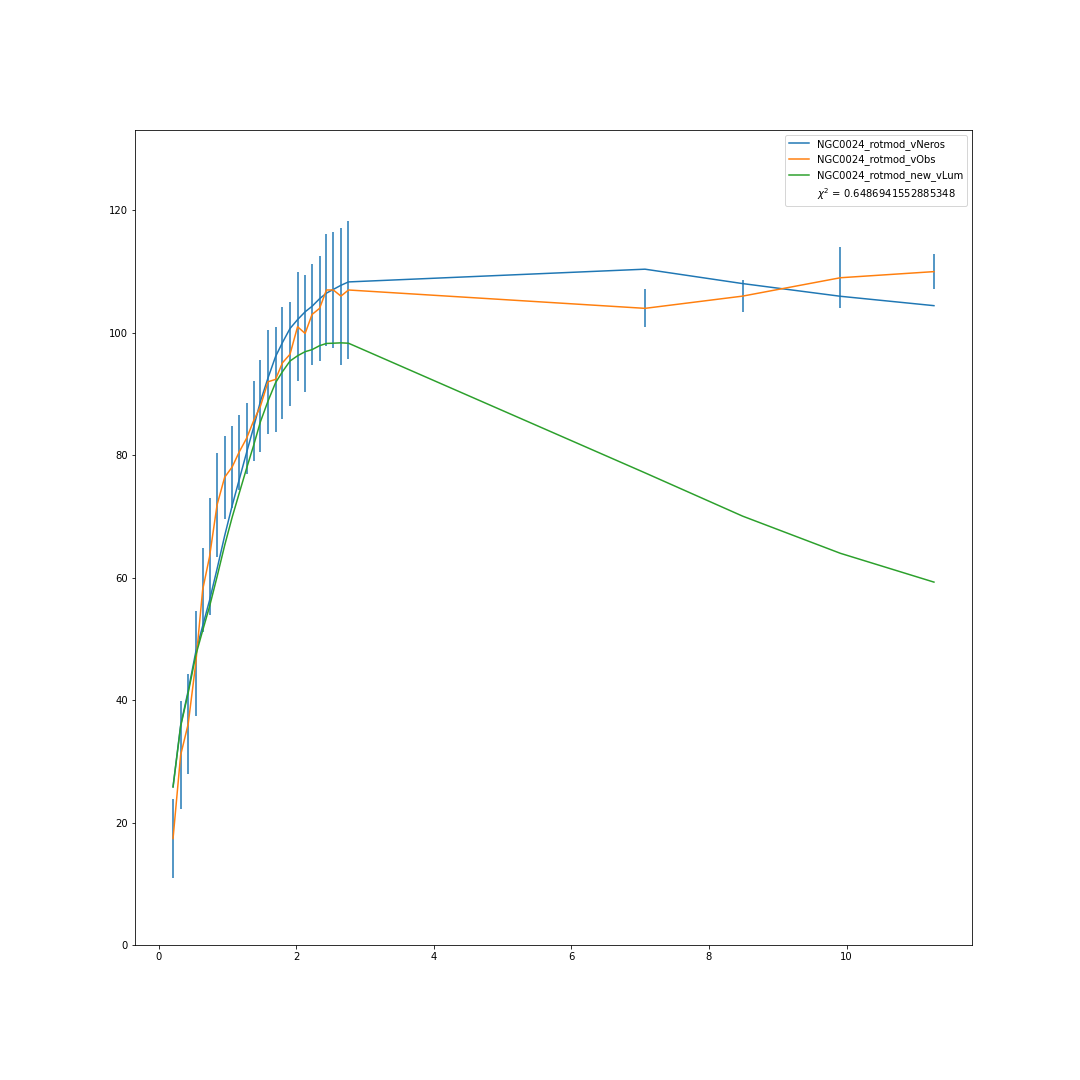
\includegraphics[width=.95\linewidth]{figures/NGC0024_rotmod_XueSofue.png}
  \captionof{figure}{ NGC0024 SPARC\cite{2016Lelli}}
  \label{fig:test2}
\end{minipage}
\begin{minipage}{.5\textwidth}
  \centering
  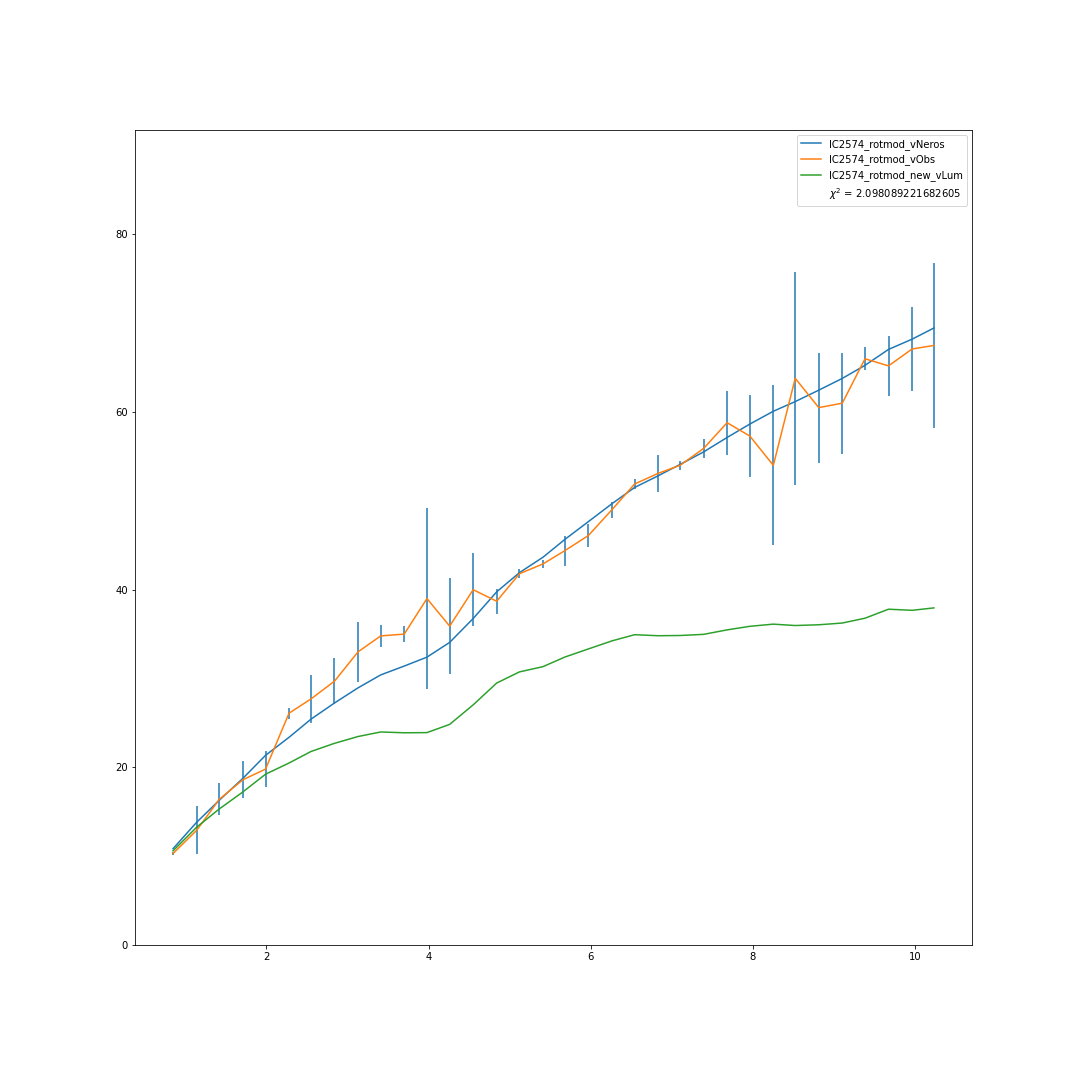
\includegraphics[width=.95\linewidth]{figures/IC2574_rotmod_XueSofue.png}
  \captionof{figure}{ IC2574  SPARC\cite{2016Lelli}}
  \label{fig:test1}
\end{minipage}%
\begin{minipage}{.5\textwidth}
  \centering
  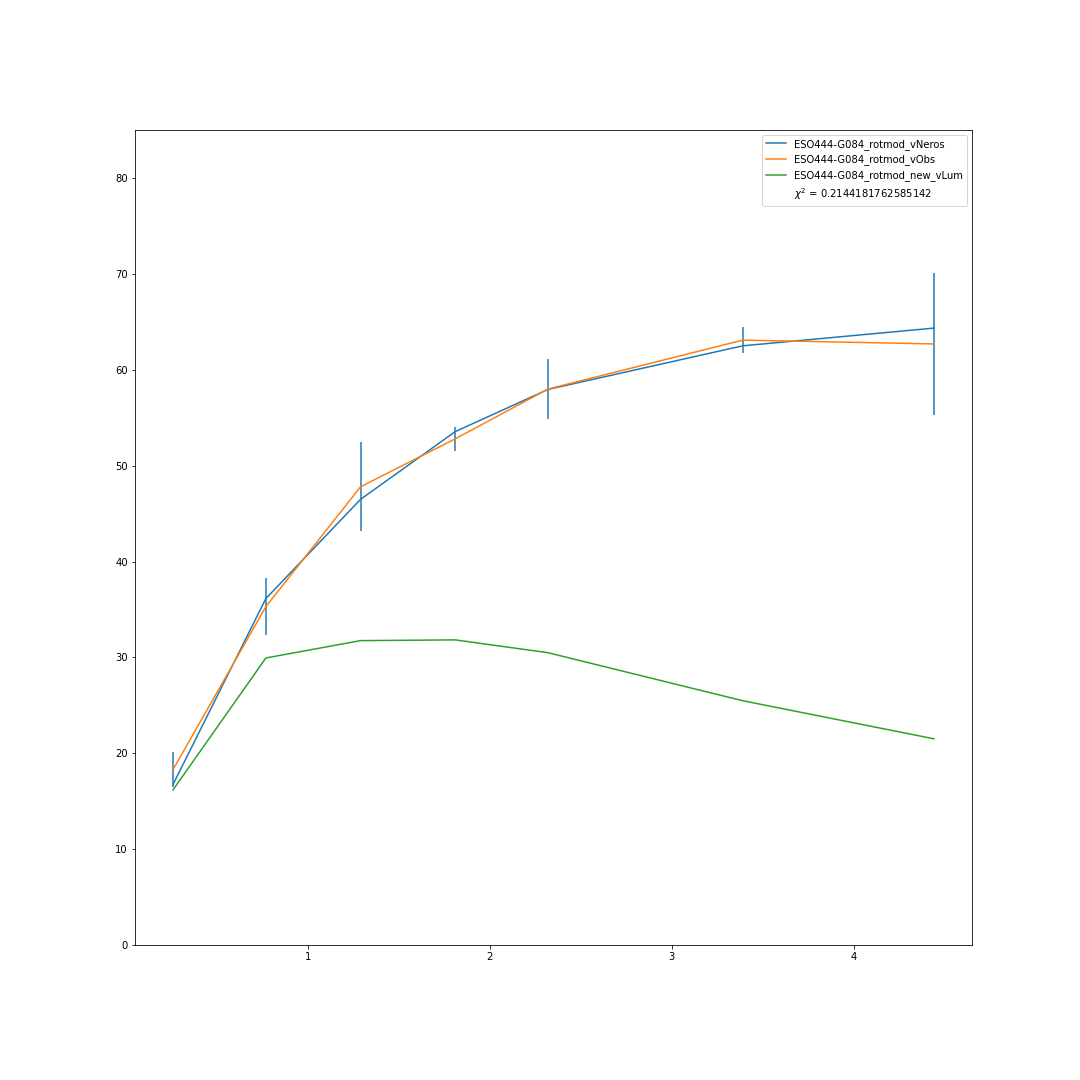
\includegraphics[width=.95\linewidth]{figures/ESO444-G084_rotmod_XueSofue.png}
  \captionof{figure}{ ESO444-G084 SPARC\cite{2016Lelli}}
  \label{fig:test1}
\end{minipage}
 \caption{Example  RCFM rotation curve fits (blue line), points with error bars are the rotation curve data, and the input baryonic mass models is  the green lines. (MARCUS PAZ : NOTE: remove orange lines, fit through data distracts from our fit)  }
\end{figure*}
 %%%%%%%
    %%%%%%%
      %%%%%%%
        %%%%%%%
          %%%%%%%
            %%%%%%%
\begin{figure*}
\centering
\begin{minipage}{.5\textwidth}
  \centering
  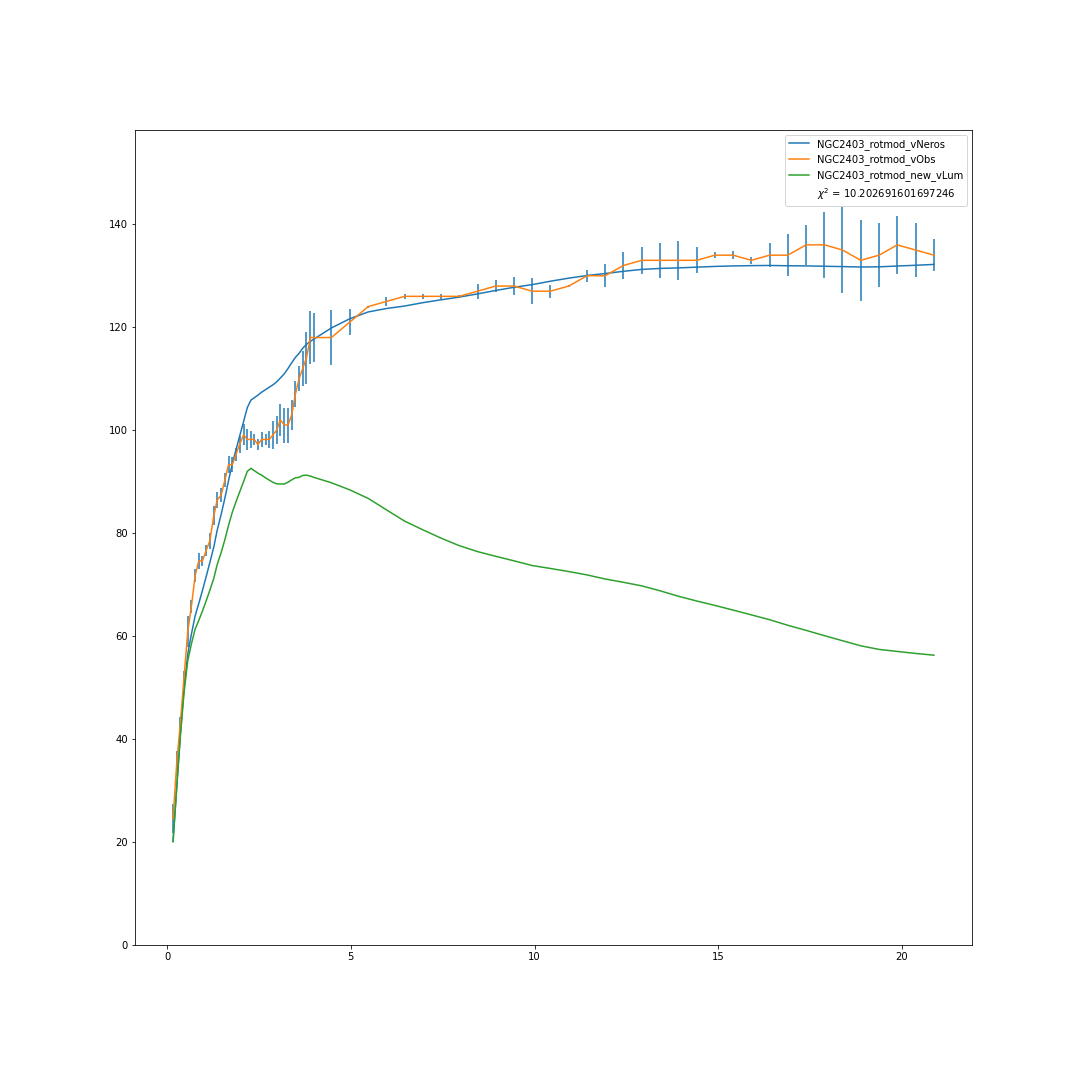
\includegraphics[width=.95\linewidth]{figures/NGC2403_rotmod_XueSofue.png}
  \captionof{figure}{ NGC2403 SPARC\cite{2016Lelli}}
  \label{fig:test1}
\end{minipage}%
\begin{minipage}{.5\textwidth}
  \centering
  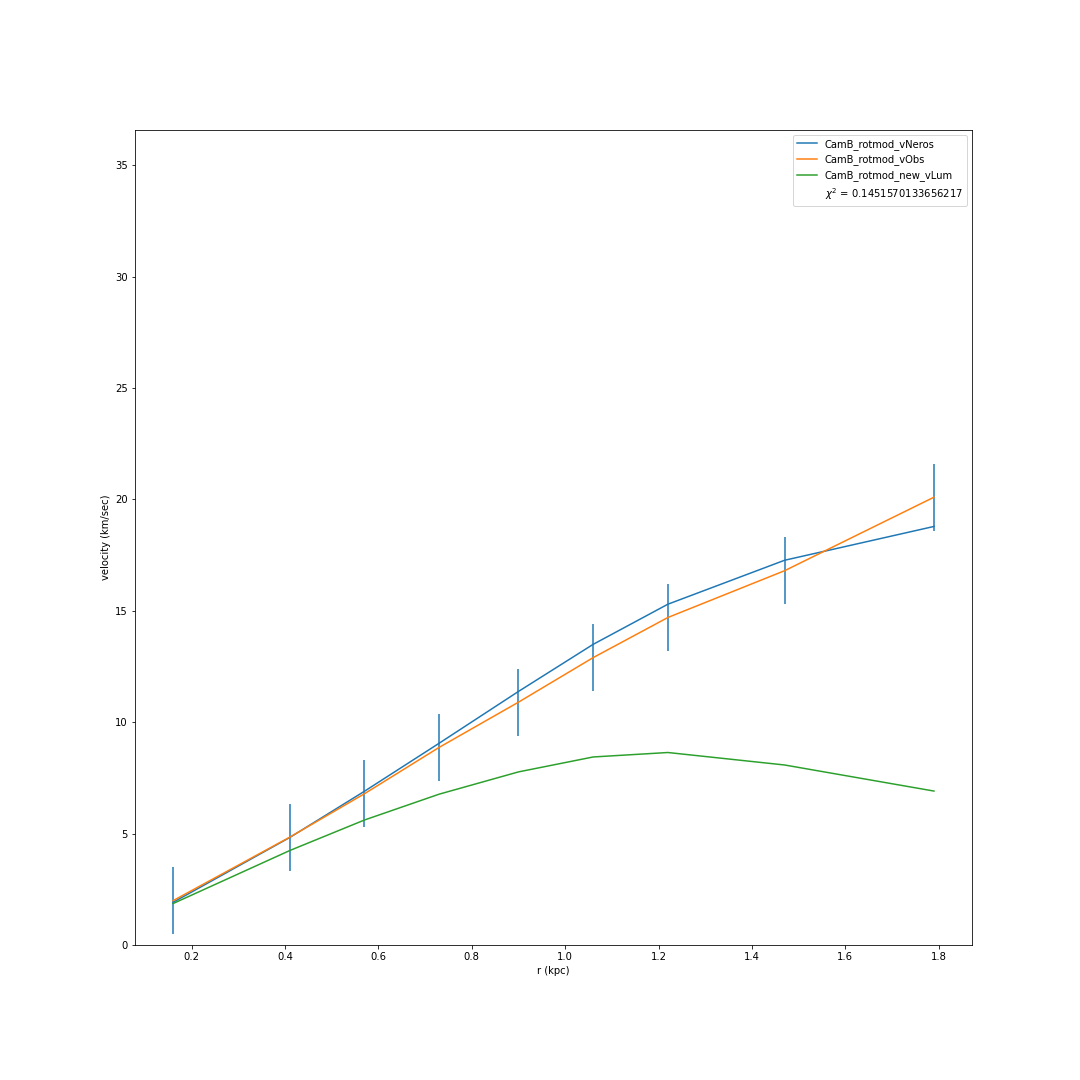
\includegraphics[width=.95\linewidth]{figures/CamB_rotmod_XueSofue.png}
  \captionof{figure}{ CamB  from SPARC\cite{2016Lelli}}
  \label{fig:test2}
\end{minipage}
\begin{minipage}{.5\textwidth}
  \centering
  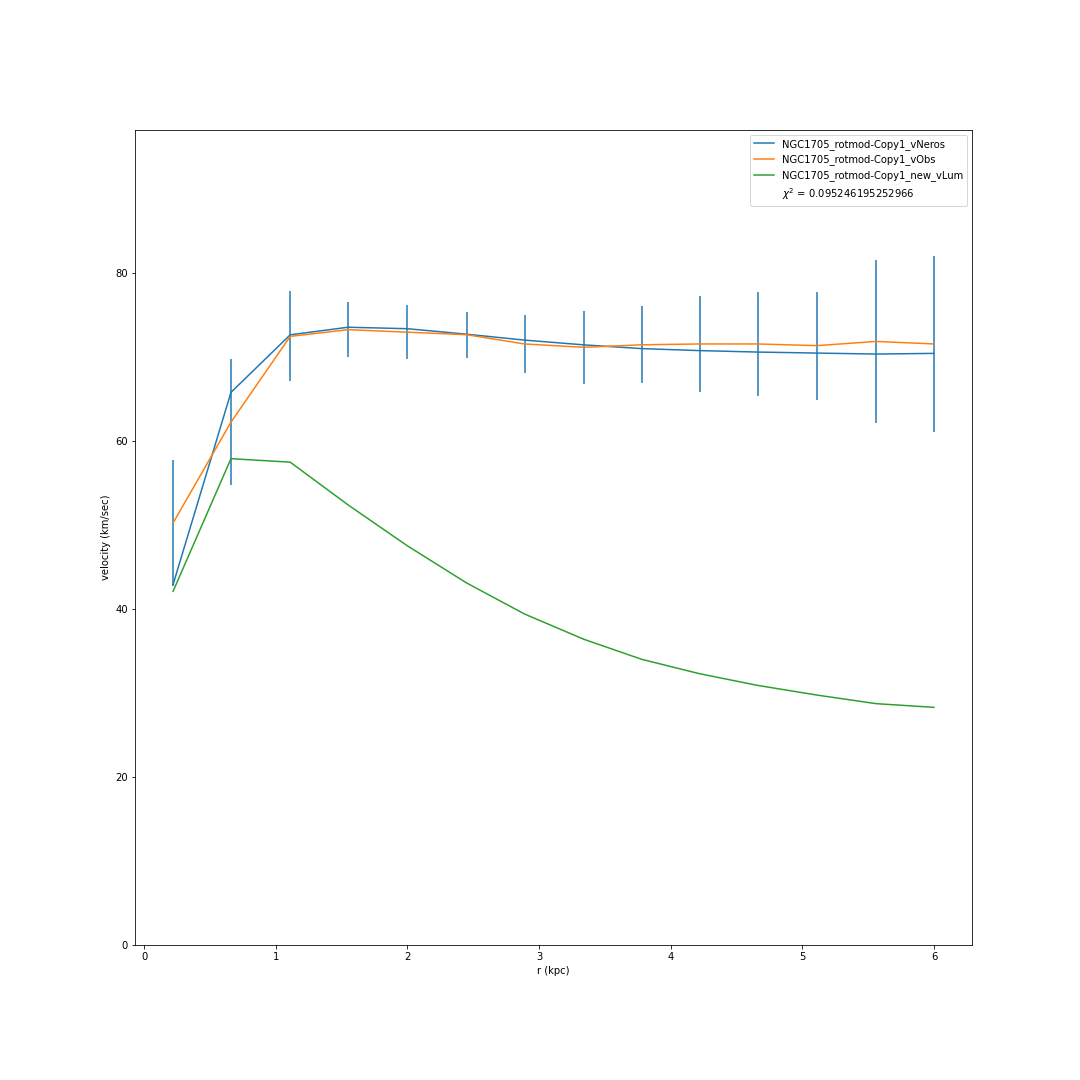
\includegraphics[width=.95\linewidth]{figures/NGC1705_rotmodXueSofue.png}
  \captionof{figure}{ NGC1705  SPARC\cite{2016Lelli}}
  \label{fig:test1}
\end{minipage}
 \caption{Example  RCFM rotation curve fits (blue), rotation curve data points with error bars (blue), and   luminous  mass models (green line). {\color{teal}NOTE: remove orange lines through data distracts, and change color of    RCFM fit to be different than data.)}  }
\end{figure*}
            %%%%%%%  %%%%%%%
  %%%%%%%   %%%%%%%  %%%%%%%
  %%%%%%%  %%%%%%%  %%%%%%%
  %%%%%%%
%%%%%%%
 %%%%%%%
 %%%%%%%
%%%%%%%
 %%%%%%%
%%%%%%%
%%%%%%%
%%%%%%%
 
 
%%%%%%%
\begin{figure} 
\centering
\begin{minipage}{0.5\textwidth}
%\centering
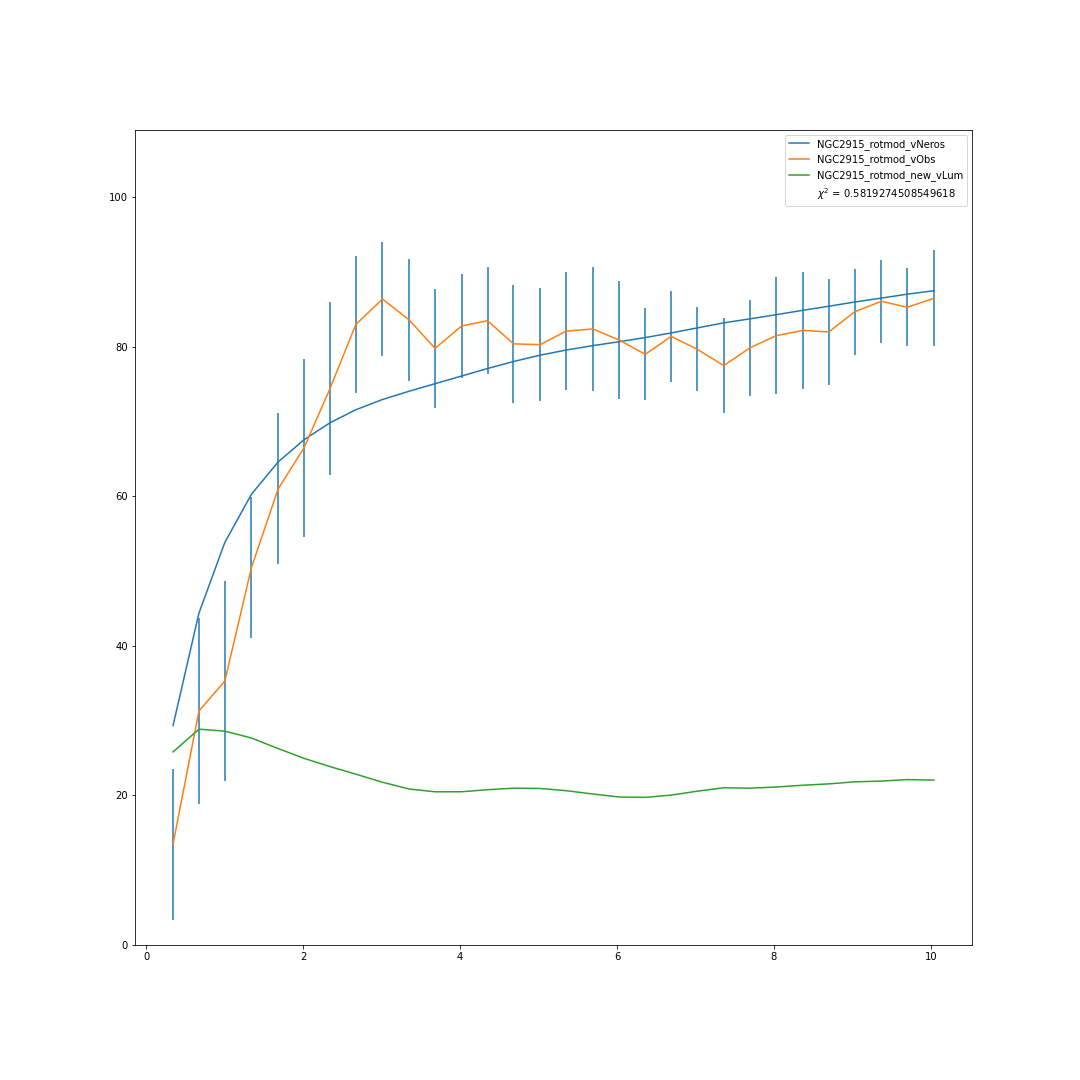
\includegraphics[width=0.95\linewidth]{figures/NGC2915_rotmod_XueSofue.png}
\caption{NGC 2915 SPARC\cite{2016Lelli}}
\label{fig:2915}
\end{minipage}
\begin{minipage}{0.5\textwidth}
%\centering
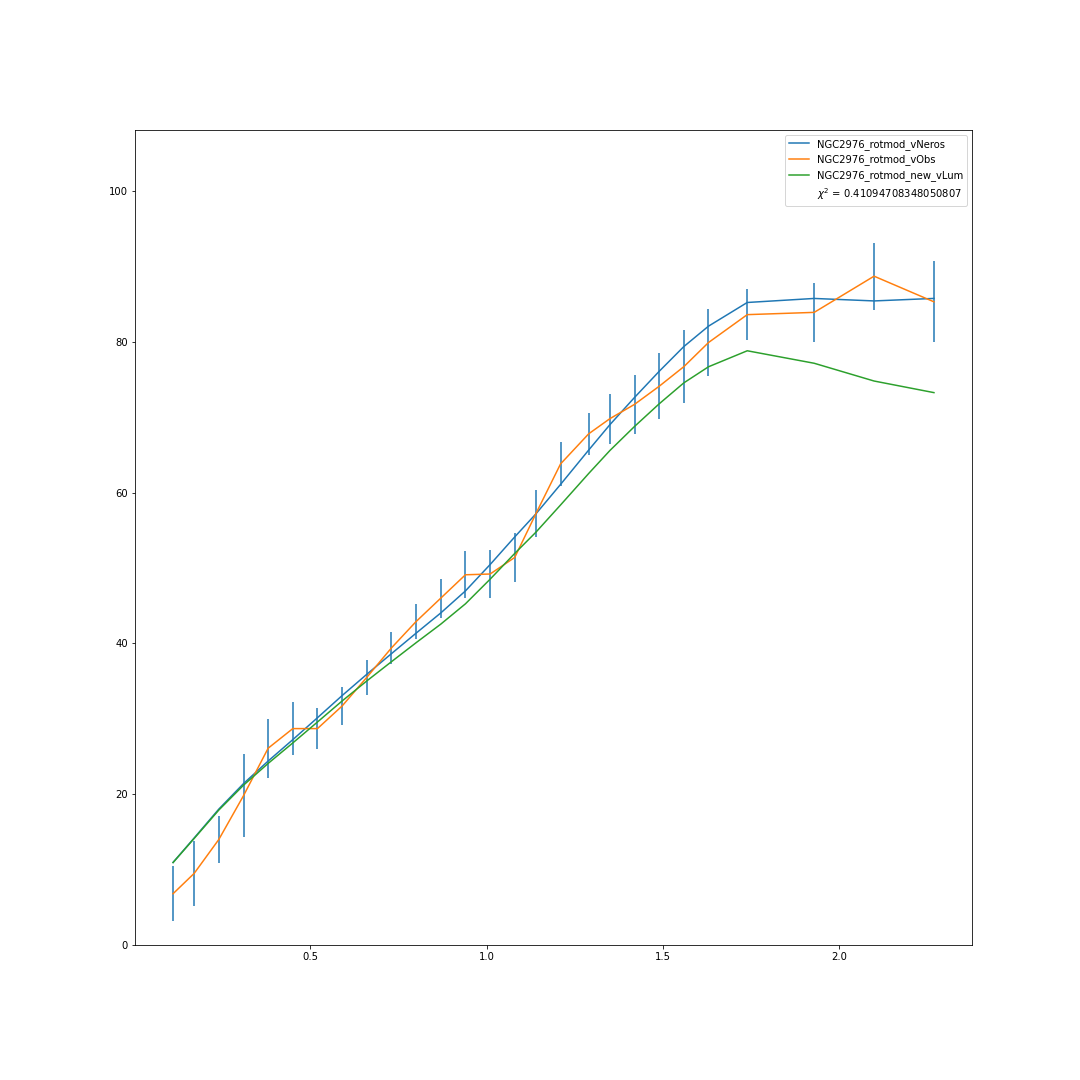
\includegraphics[width=0.95\linewidth]{figures/NGC2976_rotmod_XueSofue.png}
\caption{NGC 2976}
\label{fig:2976}
\end{minipage}
\end{figure}
%%%%%%%
%%%%%%%%
%%%%%%
%%%%%%%
%%%%%%
  
 

% Subset of galaxies to constrain RCFM free parameter }  }    \\
  \begin{table*}[]
      \centering
      \begin{tabular}{|c|c|c|c|c|c|}
      \hline \hline
\rowcolor[HTML]{CCCCCC} 
\textbf{Galaxy Name} & Hubble Type(1)& 	Distance (Mpc)&Mean Error on D (Mpc)& 	Distance Method (2)& 	Inc (deg)(3)\\
    \hline \hline\\
CamB&   	10&    3.36&  	0.26&   2&  65\\
D564-8& 	10& 	8.79& 	0.28& 	2& 	63\\
D631-7& 	10& 	7.72& 	0.18& 	2& 	59\\
DDO154& 	10& 	4.04& 	0.2& 	2& 	64\\
DDO168& 	10& 	4.25& 	0.21& 	2& 	63\\
ESO444-G084& 10& 	4.83& 	0.48& 	2& 	32\\
IC2574& 	9& 	3.91& 	0.2&    	2& 	75\\
NGC0024& 	5& 	7.3& 	0.36&   	2& 	64\\
NGC0055& 	9& 	2.11& 	0.11&   	2& 	77\\
NGC0247& 	7& 	3.7& 	0.19&   	2& 	74\\
NGC0300& 	7& 	2.08& 	0.1&    	2& 	42\\
NGC2403& 	6& 	3.16& 	0.16&   	2& 	63\\
NGC2683& 	3& 	9.81& 	0.49&   	2& 	80\\
NGC2841& 	3& 	14.1& 	1.4&    	3& 	76\\
NGC2915& 	11& 	4.06& 	0.2& 	2& 	56\\
NGC2976& 	5& 	3.58& 	0.18&   	2& 	61\\
NGC3109& 	9& 	1.33& 	0.07&   	2& 	70\\
NGC3198& 	5& 	13.8& 	1.4&    	3& 	73\\
NGC3741& 	10& 	3.21& 	0.17& 	2& 	70\\
NGC4068& 	10& 	4.37& 	0.22& 	2& 	44\\
NGC4214& 	10& 	2.87& 	0.14& 	2& 	15\\
NGC5055& 	4& 	9.9& 	0.3&    	2& 	55\\
NGC6503& 	6& 	6.26& 	0.31&   	2& 	74\\
NGC6789& 	11& 	3.52& 	0.18& 	2& 	43\\
NGC6946& 	6& 	5.52& 	1.66&   	2& 	38\\
NGC7331& 	3& 	14.7& 	1.5&    	3& 	75\\
NGC7793& 	7& 	3.61& 	0.18&   	2& 	47\\\
UGC04483& 	10& 	3.34& 	0.31& 	2& 	58\\
UGC07232& 	10& 	2.83& 	0.17& 	2& 	59\\
UGC07524& 	9& 	4.74& 	0.24& 	    2& 	46\\
UGC07559& 	10& 	4.97& 	0.25& 	2& 	61\\
UGC07577& 	10& 	2.59& 	0.13& 	2& 	63\\
UGC07866& 	10& 	4.57& 	0.23& 	2& 	44\\
UGC08490& 	9& 	4.65& 	0.53&   	2& 	50\\
UGC08837& 	10& 	7.21& 	0.36& 	2& 	80\\
UGCA442& 	9& 	4.35& 	0.22& 	    2& 	64\\
UGCA444& 	10& 	0.98& 	0.05& 	2& 	78\\
    \hline \hline           
      \end{tabular}
      \caption{{\color{blue}(UPDATED TSet on Master RCFM 2.8.23)}.
      Subset of galaxies to constrain RCFM free parameter $\alpha$.  
      (1) Hubble type 
of: 0 = S0, 1 = Sa, 2 = Sab,
3 = Sb, 4 = Sbc, 5 = Sc, 6 = Scd, 7 = Sd, 8 = Sdm,
9 = Sm, 10 = Im, 11 = BCD. 
(2) Distance method:  
2 = tip of the red giant branch, 3 = Cepheids.  (3) Inclination on the sky. All table information from \citet{2016Lelli}. } \label{tab:Tset}
  \end{table*}
 
 
 
 
\begingroup  
\setlength\extrarowheight{2pt}
\small
\setlength\LTcapwidth\textwidth
\begin{longtable*}{|c|c|c|c|c|c|c|c| }

\caption{\textbf{{\color{blue} UPDATE  TABLE }.
Comparison of Fit Results from RAR and RCFM  } } \label{table:M2Light} \\
\hline
\rowcolor[HTML]{CCCCCC} 
\textbf{Galaxy name} 
& \textbf{log (L{[}3.6{]})($L_\odot $)} 
& RAR $\gamma_{disk}$  
& RAR $\gamma_{bulge}$ 
&  RAR $\chi^2$ ave=4.22 
&\textbf{RCFM}$\chi^2$ ave=1.8
&\textbf{RCFM} $\gamma_{disk}$
&\textbf{RCFM} $\gamma_{bulge}$

\\
\hline
\endfirsthead 

\multicolumn{8}{@{}l}{\tablename~\thetable, cont'd.} \\[0.5ex]
\hline
\rowcolor[HTML]{CCCCCC} 
\textbf{Galaxy name} 
& \textbf{ (L{[}3.6{]})($10^9 L_\odot $)} 
& RAR $\gamma_{disk}$  
& RAR $\gamma_{bulge}$ 
&  RAR $\chi^2$ ave=4.22 
&\textbf{RCFM}$\chi^2$ ave=1.8
&\textbf{RCFM} $\gamma_{disk}$
&\textbf{RCFM} $\gamma_{bulge}$
 \\ \hline
\endhead 

\multicolumn{5}{r@{}}{\em Cont'd on following page}\\
\endfoot

\endlastfoot

%% Body of table
CamB                 & 7.88                      & 0.34 ± 0.08           & …                      & 5.758                                                        & 0.145                                                          & 1.43E-05                                                              & …                                                             \\
\rowcolor[HTML]{F3F3F3} 
D512-2               & 8.51                      & 0.48 ± 0.12           & …                      & 0.37                                                         & 0.052                                                       & 1.48                                                           & …                                                             \\
\rowcolor[HTML]{F3F3F3} 
D564-8               & 7.52                      & 0.40 ± 0.09           & …                      & 3.16                                                         & 0.056                                                          & 1.22                                                           & …                                                             \\
\rowcolor[HTML]{F3F3F3} 
D631-7               & 8.29                      & 0.20 ± 0.04           & …                      & 15.872                                                       & 0.242                                                         & 0.28                                                           & …                                                             \\
\rowcolor[HTML]{F3F3F3} 
DDO064               & 8.2                       & 0.48 ± 0.11           & …                      & 0.334                                                        & 0.357                                                         & 1.58                                                           & …                                                             \\
\rowcolor[HTML]{F3F3F3} 
DDO154               & 7.72                      & 0.19 ± 0.03           & …                      & 3.482                                                        & 8.155                                                            & 1.20                                                          & …                                                             \\
\rowcolor[HTML]{F3F3F3} 
DDO161               & 8.74                      & 0.23 ± 0.04           & …                      & 1.468                                                        & 0.585                                                         & 0.98                                                           & …                                                             \\
\rowcolor[HTML]{F3F3F3} 
DDO168               & 8.28                      & 0.46 ± 0.11           & …                      & 19.714                                                       & 3.087                                                           & 0.79                                                          & …                                                             \\
\rowcolor[HTML]{F3F3F3} 
DDO170               & 8.73                      & 0.79 ± 0.15           & …                      & 4.917                                                        & 2.006                                                            & 1.84                                                           & …                                                             \\
\rowcolor[HTML]{F3F3F3} 
ESO079-G014          & 10.71                     & 0.50 ± 0.09           & …                      & 4.334                                                        & 3.081                                                          & 1.09                                                            & …                                                             \\
\rowcolor[HTML]{F3F3F3} 
ESO116-G012          & 9.63                      & 0.35 ± 0.04           & …                      & 2.444                                                        & 0.842                                                        & 1.04                                                          & …                                                             \\
\rowcolor[HTML]{F3F3F3} 
ESO444-G084          & 7.85                      & 0.42 ± 0.09           & …                      & 3.253                                                        & 0.214                                                          & 1.87                                                           & …                                                             \\
\rowcolor[HTML]{F3F3F3} 
ESO563-G021          & 11.49                     & 0.43 ± 0.04           & …                      & 28.836                                                       & 14.570                                                          & 0.99                                                          & …                                                             \\
\rowcolor[HTML]{F3F3F3} 
F561-1               & 9.61                      & 0.52 ± 0.13           & …                      & 1.564                                                        & 0.525                                                          & 0.96                                                          & …                                                             \\
\rowcolor[HTML]{F3F3F3} 
F563-1               & 9.28                      & 0.56 ± 0.12           & …                      & 1.499                                                        & 0.788                                                         & 2.07                                                           & …                                                             \\
\rowcolor[HTML]{F3F3F3} 
F563-V1              & 9.19                      & 0.48 ± 0.12           & …                      & 0.875                                                        & 0.143                                                         & 0.99                                                           & …                                                             \\
\rowcolor[HTML]{F3F3F3} 
F563-V2              & 9.48                      & 0.59 ± 0.14           & …                      & 0.991                                                        & 0.079                                                       & 2.20                                                           & …                                                             \\
\rowcolor[HTML]{F3F3F3} 
F565-V2              & 8.75                      & 0.50 ± 0.12           & …                      & 0.474                                                        & 0.181                                                        & 2.23                                                           & …                                                             \\
\rowcolor[HTML]{F3F3F3} 
F567-2               & 9.33                      & 0.56 ± 0.13           & …                      & 2.204                                                        & 0.200                                                       & 1.31                                                           & …                                                             \\
\rowcolor[HTML]{F3F3F3} 
F568-1               & 9.8                       & 0.61 ± 0.13           & …                      & 1.287                                                        & 0.539                                                        & 1.91                                                            & …                                                             \\
\rowcolor[HTML]{F3F3F3} 
F568-3               & 9.92                      & 0.41 ± 0.09           & …                      & 3.064                                                        & 1.500                                                          & 1.31                                                           & …                                                             \\
\rowcolor[HTML]{F3F3F3} 
F568-V1              & 9.58                      & 0.81 ± 0.16           & …                      & 1.042                                                        & 0.109                                                         & 2.14                                                           & …                                                             \\
\rowcolor[HTML]{F3F3F3} 
F571-8               & 10.01                     & 0.11 ± 0.02           & …                      & 41.61                                                        & 1.550                                                        & 0.18                                                          & …                                                             \\
\rowcolor[HTML]{F3F3F3} 
F571-V1              & 9.27                      & 0.50 ± 0.12           & …                      & 0.288                                                        & 0.116                                                          & 1.49                                                         & …                                                             \\
\rowcolor[HTML]{F3F3F3} 
F574-1               & 9.82                      & 0.71 ± 0.13           & …                      & 2.501                                                        & 1.125                                                           & 1.54                                                           & …                                                             \\
\rowcolor[HTML]{F3F3F3} 
F574-2               & 9.46                      & 0.49 ± 0.12           & …                      & 0.092                                                        & 0.0559                                                         & 0.67                                                          & …                                                             \\
\rowcolor[HTML]{F3F3F3} 
F579-V1              & 10.07                     & 0.63 ± 0.14           & …                      & 2.559                                                        & 0.844                                                         & 1.63                                                           & …                                                             \\
\rowcolor[HTML]{F3F3F3} 
F583-1               & 8.99                      & 0.91 ± 0.14           & …                      & 2.663                                                        & 0.926                                                          & 1.87                                                            & …                                                             \\
\rowcolor[HTML]{F3F3F3} 
F583-4               & 9.23                      & 0.48 ± 0.11           & …                      & 0.134                                                        & 0.208                                                          & 1.30                                                           & …                                                             \\
\rowcolor[HTML]{F3F3F3} 
IC2574               & 9.01                      & 0.07 ± 0.00           & …                      & 1.44                                                         & 2.098                                                          & 1.11                                                           & …                                                             \\
\rowcolor[HTML]{F3F3F3} 
IC4202               & 11.25                     & 1.60 ± 0.19           & 0.34 ± 0.04            & 41.908                                                       & 11.571                                                         & 6.28E-06                                                              & \multicolumn{1}{r}{\cellcolor[HTML]{F3F3F3}0.4487872394}      \\
\rowcolor[HTML]{F3F3F3} 
KK98-251             & 7.93                      & 0.44 ± 0.10           & …                      & 1.227                                                        & 0.336                                                         & 1.67                                                          & …                                                             \\
\rowcolor[HTML]{F3F3F3} 
NGC0024              & 9.59                      & 1.01 ± 0.11           & …                      & 0.85                                                         & 0.649                                                          & 1.39                                                          & …                                                             \\
\rowcolor[HTML]{F3F3F3} 
NGC0055              & 9.67                      & 0.19 ± 0.03           & …                      & 1.579                                                        & 2.508                                                            & 1.02                                                           & …                                                             \\
\rowcolor[HTML]{F3F3F3} 
NGC0100              & 9.51                      & 0.28 ± 0.06           & …                      & 1.286                                                        & 0.089                                                        & 0.93                                                          & …                                                             \\
\rowcolor[HTML]{F3F3F3} 
NGC0247              & 9.87                      & 0.78 ± 0.08           & …                      & 3.06                                                         & 1.925                                                        & 1.53                                                           & …                                                             \\
\rowcolor[HTML]{F3F3F3} 
NGC0289              & 10.86                     & 0.92 ± 0.09           & …                      & 2.132                                                        & 1.563                                                          & 0.74                                                            & …                                                             \\
\rowcolor[HTML]{F3F3F3} 
NGC0300              & 9.47                      & 0.40 ± 0.05           & …                      & 0.906                                                        & 0.374                                                          & 1.14                                                           & …                                                             \\
\rowcolor[HTML]{F3F3F3} 
NGC0801              & 11.49                     & 1.33 ± 0.12           & …                      & 7.753                                                        & 5.886                                                          & 0.76                                                          & …                                                             \\
\rowcolor[HTML]{F3F3F3} 
NGC0891              & 11.14                     & 0.33 ± 0.02           & 0.40 ± 0.05            & 7.368                                                        & 2.983                                                          & 0.42                                                          & \multicolumn{1}{r}{\cellcolor[HTML]{F3F3F3}0.7485043087}      \\
\rowcolor[HTML]{F3F3F3} 
NGC1003              & 9.83                      & 0.37 ± 0.03           & …                      & 4.669                                                        & 2.951                                                         & 0.78                                                          & …                                                             \\
\rowcolor[HTML]{F3F3F3} 
NGC1090              & 10.86                     & 0.74 ± 0.07           & …                      & 2.778                                                        & 1.985                                                          & 0.81                                                         & …                                                             \\
\rowcolor[HTML]{F3F3F3} 
NGC1705              & 8.73                      & 1.22 ± 0.13           & …                      & 0.373                                                        & 0.095                                                       & 1.25                                                           & …                                                             \\
\rowcolor[HTML]{F3F3F3} 
NGC2366              & 8.37                      & 0.24 ± 0.03           & …                      & 1.934                                                        & 2.108                                                         & 1.06                                                           & …                                                             \\
\rowcolor[HTML]{F3F3F3} 
NGC2403              & 10                        & 0.51 ± 0.01           & …                      & 14.142                                                       & 10.203                                                          & 0.86                                                          & …                                                             \\
\rowcolor[HTML]{F3F3F3} 
NGC2683              & 10.91                     & 0.55 ± 0.06           & 0.73 ± 0.18            & 3.37                                                         & 0.737                                                          & 0.88                                                          & \multicolumn{1}{r}{\cellcolor[HTML]{F3F3F3}0.4235079131}      \\
\rowcolor[HTML]{F3F3F3} 
NGC2841              & 11.27                     & 0.81 ± 0.05           & 0.93 ± 0.05            & 1.515                                                        & 1.299                                                            & 0.87                                                          & \multicolumn{1}{r}{\cellcolor[HTML]{F3F3F3}1.105158794}       \\
\rowcolor[HTML]{F3F3F3} 
NGC2903              & 10.91                     & 0.21 ± 0.01           & …                      & 20.637                                                       & 6.904                                                          & 0.62                                                           & …                                                             \\
\rowcolor[HTML]{F3F3F3} 
NGC2915              & 8.81                      & 0.32 ± 0.05           & …                      & 4.017                                                        & 0.582                                                          & 0.57                                                          & …                                                             \\
\rowcolor[HTML]{F3F3F3} 
NGC2955              & 11.5                      & 0.37 ± 0.06           & 0.84 ± 0.08            & 3.906                                                        & 4.058                                                             & 0.38                                                           & \multicolumn{1}{r}{\cellcolor[HTML]{F3F3F3}0.873021573}       \\
\rowcolor[HTML]{F3F3F3} 
NGC2976              & 9.53                      & 0.35 ± 0.08           & …                      & 1.73                                                         & 0.411                                                          & 0.91                                                          & …                                                             \\
\rowcolor[HTML]{F3F3F3} 
NGC2998              & 11.18                     & 0.82 ± 0.10           & …                      & 2.94                                                         & 2.918                                                         & 0.87                                                          & …                                                             \\
\rowcolor[HTML]{F3F3F3} 
NGC3109              & 8.29                      & 0.21 ± 0.04           & …                      & 4.133                                                        & 0.245                                                          & 2.05                                                            & …                                                             \\
\rowcolor[HTML]{F3F3F3} 
NGC3198              & 10.58                     & 0.77 ± 0.03           & …                      & 2.057                                                        & 1.676                                                           & 0.88                                                          & …                                                             \\
\rowcolor[HTML]{F3F3F3} 
NGC3521              & 10.93                     & 0.46 ± 0.05           & …                      & 0.51                                                         & 0.732                                                          & 0.70                                                          & …                                                             \\
\rowcolor[HTML]{F3F3F3} 
NGC3726              & 10.85                     & 0.47 ± 0.07           & …                      & 2.982                                                        & 1.798                                                          & 0.76                                                          & …                                                             \\
\rowcolor[HTML]{F3F3F3} 
NGC3741              & 7.45                      & 0.31 ± 0.05           & …                      & 0.767                                                        & 0.546                                                          & 0.72                                                           & …                                                             \\
\rowcolor[HTML]{F3F3F3} 
NGC3769              & 10.27                     & 0.41 ± 0.07           & …                      & 0.949                                                        & 0.568                                                           & 0.71                                                          & …                                                             \\
\rowcolor[HTML]{F3F3F3} 
NGC3877              & 10.86                     & 0.40 ± 0.07           & …                      & 10.221                                                       & 6.979                                                          & 0.87                                                          & …                                                             \\
\rowcolor[HTML]{F3F3F3} 
NGC3893              & 10.77                     & 0.45 ± 0.06           & …                      & 0.997                                                        & 0.402                                                        & 0.73                                                       & …                                                             \\
\rowcolor[HTML]{F3F3F3} 
NGC3917              & 10.34                     & 0.55 ± 0.09           & …                      & 4.603                                                        & 2.218                                                           & 1.14                                                          & …                                                             \\
\rowcolor[HTML]{F3F3F3} 
NGC3949              & 10.58                     & 0.44 ± 0.07           & …                      & 0.547                                                        & 0.435                                                         & 0.73                                                          & …                                                             \\
\rowcolor[HTML]{F3F3F3} 
NGC3953              & 11.15                     & 0.59 ± 0.10           & …                      & 3.424                                                        & 0.474                                                       & 0.90                                                          & …                                                             \\
\rowcolor[HTML]{F3F3F3} 
NGC3972              & 10.16                     & 0.50 ± 0.08           & …                      & 2.074                                                        & 1.459                                                          & 1.03                                                           & …                                                             \\
\rowcolor[HTML]{F3F3F3} 
NGC3992              & 11.36                     & 0.76 ± 0.10           & …                      & 3.465                                                        & 1.181                                                         & 1.04                                                          & …                                                             \\
\rowcolor[HTML]{F3F3F3} 
NGC4010              & 10.24                     & 0.36 ± 0.07           & …                      & 2.741                                                        & 1.429                                                         & 0.85                                                         & …                                                             \\
\rowcolor[HTML]{F3F3F3} 
NGC4013              & 10.9                      & 0.35 ± 0.05           & 0.79 ± 0.17            & 1.807                                                        & 1.379                                                          & 0.55                                                         & \multicolumn{1}{r}{\cellcolor[HTML]{F3F3F3}1.428297479}       \\
\rowcolor[HTML]{F3F3F3} 
NGC4051              & 10.98                     & 0.45 ± 0.09           & …                      & 2.491                                                        & 1.087                                                         & 0.81                                                          & …                                                             \\
\rowcolor[HTML]{F3F3F3} 
NGC4068              & 8.37                      & 0.38 ± 0.09           & …                      & 2.519                                                        & 0.138                                                         & 0.80                                                          & …                                                             \\
\rowcolor[HTML]{F3F3F3} 
NGC4085              & 10.34                     & 0.35 ± 0.06           & …                      & 9.088                                                        & 1.623                                                          & 0.58                                                         & …                                                             \\
\rowcolor[HTML]{F3F3F3} 
NGC4088              & 11.03                     & 0.40 ± 0.07           & …                      & 0.664                                                        & 0.650                                                         & 0.63                                                         & …                                                             \\
\rowcolor[HTML]{F3F3F3} 
NGC4100              & 10.77                     & 0.76 ± 0.10           & …                      & 1.658                                                        & 1.672                                                           & 0.95                                                         & …                                                             \\
\rowcolor[HTML]{F3F3F3} 
NGC4138              & 10.64                     & 0.55 ± 0.11           & 0.69 ± 0.17            & 2.492                                                        & 0.424                                                          & 0.98                                                          & \multicolumn{1}{r}{\cellcolor[HTML]{F3F3F3}6.18E-05}          \\
\rowcolor[HTML]{F3F3F3} 
NGC4157              & 11.02                     & 0.43 ± 0.06           & 0.64 ± 0.15            & 0.72                                                         & 0.489                                                         & 0.69                                                         & \multicolumn{1}{r}{\cellcolor[HTML]{F3F3F3}0.5628009768}      \\
\rowcolor[HTML]{F3F3F3} 
NGC4183              & 10.03                     & 0.79 ± 0.14           & …                      & 1.132                                                        & 0.457                                                        & 1.25                                                           & …                                                             \\
\rowcolor[HTML]{F3F3F3} 
NGC4214              & 9.06                      & 0.46 ± 0.11           & …                      & 1.062                                                        & 0.925                                                           & 1.02                                                          & …                                                             \\
\rowcolor[HTML]{F3F3F3} 
NGC4217              & 10.93                     & 1.17 ± 0.20           & 0.17 ± 0.02            & 3.171                                                        & 1.118                                                           & 1.13                                                           & \multicolumn{1}{r}{\cellcolor[HTML]{F3F3F3}0.4552799494}      \\
\rowcolor[HTML]{F3F3F3} 
NGC4389              & 10.33                     & 0.30 ± 0.07           & …                      & 9.313                                                        & 0.104                                                          & 0.31                                                          & …                                                             \\
\rowcolor[HTML]{F3F3F3} 
NGC4559              & 10.29                     & 0.52 ± 0.06           & …                      & 0.496                                                        & 0.318                                                          & 0.77                                                           & …                                                             \\
\rowcolor[HTML]{F3F3F3} 
NGC5005              & 11.25                     & 0.54 ± 0.07           & 0.56 ± 0.07            & 0.091                                                        & 0.065                                                         & 0.59                                                           & \multicolumn{1}{r}{\cellcolor[HTML]{F3F3F3}0.6849763505}      \\
\rowcolor[HTML]{F3F3F3} 
NGC5033              & 11.04                     & 1.03 ± 0.08           & 0.43 ± 0.06            & 8.024                                                        & 5.535                                                          & 0.84                                                           & \multicolumn{1}{r}{\cellcolor[HTML]{F3F3F3}0.5157817709}      \\
\rowcolor[HTML]{F3F3F3} 
NGC5055              & 11.18                     & 0.56 ± 0.01           & …                      & 7.415                                                        & 6.028                                                           & 0.62                                                          & …                                                             \\
\rowcolor[HTML]{F3F3F3} 
NGC5371              & 11.53                     & 3.30 ± 0.29           & …                      & 10.156                                                       & 10.587                                                           & 0.77                                                          & …                                                             \\
\rowcolor[HTML]{F3F3F3} 
NGC5585              & 9.47                      & 0.22 ± 0.01           & …                      & 6.817                                                        & 5.503                                                           & 0.75                                                           & …                                                             \\
\rowcolor[HTML]{F3F3F3} 
NGC5907              & 11.24                     & 1.08 ± 0.07           & …                      & 7.73                                                         & 6.768                                                          & 0.93                                                          & …                                                             \\
\rowcolor[HTML]{F3F3F3} 
NGC5985              & 11.32                     & 0.63 ± 0.10           & 3.32 ± 0.30            & 6.974                                                        & 5.165                                                           & 0.95                                                           & \multicolumn{1}{r}{\cellcolor[HTML]{F3F3F3}2.132734768}       \\
\rowcolor[HTML]{F3F3F3} 
NGC6015              & 10.51                     & 1.12 ± 0.06           & …                      & 10.873                                                       & 12.088                                                           & 0.99                                                           & …                                                             \\
\rowcolor[HTML]{F3F3F3} 
NGC6195              & 11.59                     & 0.32 ± 0.06           & 0.85 ± 0.07            & 2.258                                                        & 2.709                                                           & 0.37                                                          & \multicolumn{1}{r}{\cellcolor[HTML]{F3F3F3}0.8051651041}      \\
\rowcolor[HTML]{F3F3F3} 
NGC6503              & 10.11                     & 0.45 ± 0.02           & …                      & 2.979                                                        & 1.418                                                         & 0.75                                                           & …                                                             \\
\rowcolor[HTML]{F3F3F3} 
NGC6674              & 11.33                     & 0.95 ± 0.11           & 1.30 ± 0.45            & 10.638                                                       & 2.969                                                         & 0.67                                                          & \multicolumn{1}{r}{\cellcolor[HTML]{F3F3F3}1.807748783}       \\
\rowcolor[HTML]{F3F3F3} 
NGC6789              & 8                         & 0.60 ± 0.14           & …                      & 5.904                                                        & 0.143                                                        & 1.41                                                         & …                                                             \\
\rowcolor[HTML]{F3F3F3} 
NGC6946              & 10.82                     & 0.64 ± 0.05           & 0.71 ± 0.04            & 1.525                                                        & 1.682                                                          & 0.64                                                           & \multicolumn{1}{r}{\cellcolor[HTML]{F3F3F3}0.5735330606}      \\
\rowcolor[HTML]{F3F3F3} 
NGC7331              & 11.4                      & 0.32 ± 0.02           & 0.60 ± 0.12            & 1.289                                                        & 0.962                                                          & 0.51                                                          & \multicolumn{1}{r}{\cellcolor[HTML]{F3F3F3}1.201353002}       \\
\rowcolor[HTML]{F3F3F3} 
NGC7793              & 9.85                      & 0.55 ± 0.09           & …                      & 1.013                                                        & 0.701                                                         & 0.89                                                          & …                                                             \\
\rowcolor[HTML]{F3F3F3} 
NGC7814              & 10.87                     & 1.17 ± 0.12           & 0.52 ± 0.04            & 1.334                                                        & 0.533                                                         & 0.42                                                          & \multicolumn{1}{r}{\cellcolor[HTML]{F3F3F3}0.6735053081}      \\
\rowcolor[HTML]{F3F3F3} 
PGC51017             & 8.19                      & 0.44 ± 0.10           & …                      & 4.567                                                        & 1.156                                                         & 0.80                                                          & …                                                             \\
\rowcolor[HTML]{F3F3F3} 
UGC00128             & 10.08                     & 2.49 ± 0.12           & …                      & 6.254                                                        & 5.326                                                           & 1.65                                                           & …                                                             \\
\rowcolor[HTML]{F3F3F3} 
UGC00191             & 9.3                       & 1.10 ± 0.13           & …                      & 3.842                                                        & 1.628                                                           & 1.38                                                          & …                                                             \\
\rowcolor[HTML]{F3F3F3} 
UGC00634             & 9.48                      & 0.49 ± 0.09           & …                      & 2.425                                                        & 1.561                                                          & 1.57                                                            & …                                                             \\
\rowcolor[HTML]{F3F3F3} 
UGC00731             & 8.51                      & 2.39 ± 0.45           & …                      & 6.415                                                        & 0.062                                                         & 3.79                                                           & …                                                             \\
\rowcolor[HTML]{F3F3F3} 
UGC00891             & 8.57                      & 0.32 ± 0.07           & …                      & 25.16                                                        & 0.613                                                          & 1.35                                                           & …                                                             \\
\rowcolor[HTML]{F3F3F3} 
UGC01230             & 9.88                      & 0.72 ± 0.17           & …                      & 2.951                                                        & 0.588                                                         & 1.72                                                           & …                                                             \\
\rowcolor[HTML]{F3F3F3} 
UGC01281             & 8.55                      & 0.39 ± 0.06           & …                      & 0.244                                                        & 0.299                                                          & 1.43                                                         & …                                                             \\
\rowcolor[HTML]{F3F3F3} 
UGC02023             & 9.12                      & 0.49 ± 0.12           & …                      & 1.147                                                        & 0.022                                                         & 0.72                                                        & …                                                             \\
\rowcolor[HTML]{F3F3F3} 
UGC02259             & 9.24                      & 1.14 ± 0.19           & …                      & 7.221                                                        & 2.896                                                          & 1.82                                                          & …                                                             \\
\rowcolor[HTML]{F3F3F3} 
UGC02455             & 9.56                      & 0.33 ± 0.09           & …                      & 6.549                                                        & 0.560                                                         & 0.28                                                         & …                                                             \\
\rowcolor[HTML]{F3F3F3} 
UGC02487             & 11.69                     & 1.83 ± 0.20           & 0.91 ± 0.18            & 4.482                                                        & 3.036                                                         & 1.16                                                           & \multicolumn{1}{r}{\cellcolor[HTML]{F3F3F3}0.9115559635}      \\
\rowcolor[HTML]{F3F3F3} 
UGC02885             & 11.61                     & 0.45 ± 0.06           & 0.97 ± 0.08            & 0.858                                                        & 1.958                                                          & 0.44                                                           & \multicolumn{1}{r}{\cellcolor[HTML]{F3F3F3}0.9616477641}      \\
\rowcolor[HTML]{F3F3F3} 
UGC02916             & 11.09                     & 1.57 ± 0.24           & 0.73 ± 0.06            & 11.652                                                       & 10.632                                                          & 1.43                                                          & \multicolumn{1}{r}{\cellcolor[HTML]{F3F3F3}0.7041612394}      \\
\rowcolor[HTML]{F3F3F3} 
UGC02953             & 11.41                     & 0.61 ± 0.01           & 0.62 ± 0.01            & 5.661                                                        & \multicolumn{1}{l}{\cellcolor[HTML]{F3F3F3}fails}                     & 1                                                                     & 1                                                             \\
\rowcolor[HTML]{F3F3F3} 
UGC03205             & 11.06                     & 0.73 ± 0.06           & 1.32 ± 0.07            & 4.196                                                        & 2.720                                                        & 0.68                                                         & \multicolumn{1}{r}{\cellcolor[HTML]{F3F3F3}1.056511275}       \\
\rowcolor[HTML]{F3F3F3} 
UGC03546             & 11.01                     & 0.68 ± 0.08           & 0.51 ± 0.04            & 0.907                                                        & 1.040                                                         & 0.62                                                          & \multicolumn{1}{r}{\cellcolor[HTML]{F3F3F3}0.5984123234}      \\
\rowcolor[HTML]{F3F3F3} 
UGC03580             & 10.12                     & 0.29 ± 0.02           & 0.11 ± 0.01            & 2.291                                                        & 2.014                                                         & 0.52                                                          & \multicolumn{1}{r}{\cellcolor[HTML]{F3F3F3}0.4156621765}      \\
\rowcolor[HTML]{F3F3F3} 
UGC04278             & 9.12                      & 0.53 ± 0.07           & …                      & 2.597                                                        & 0.795                                                          & 1.01                                                          & …                                                             \\
\rowcolor[HTML]{F3F3F3} 
UGC04305             & 8.87                      & 0.71 ± 0.16           & …                      & 2.024                                                        & 1.552                                                        & 0.88                                                           & …                                                             \\
\rowcolor[HTML]{F3F3F3} 
UGC04325             & 9.31                      & 0.94 ± 0.19           & …                      & 9.429                                                        & 2.326                                                           & 1.87                                                           & …                                                             \\
\rowcolor[HTML]{F3F3F3} 
UGC04483             & 7.11                      & 0.43 ± 0.10           & …                      & 0.869                                                        & 0.326                                                          & 1.28                                                           & …                                                             \\
\rowcolor[HTML]{F3F3F3} 
UGC04499             & 9.19                      & 0.51 ± 0.10           & …                      & 1.776                                                        & 1.040                                                         & 1.15                                                           & …                                                             \\
\rowcolor[HTML]{F3F3F3} 
UGC05005             & 9.61                      & 0.45 ± 0.10           & …                      & 0.315                                                        & 0.070c                                                       & 1.04                                                            & …                                                             \\
\rowcolor[HTML]{F3F3F3} 
UGC05253             & 11.23                     & 0.63 ± 0.05           & 0.69 ± 0.03            & 4.747                                                        & 5.519                                                       & 0.51                                                           & \multicolumn{1}{r}{\cellcolor[HTML]{F3F3F3}0.7071814094}      \\
\rowcolor[HTML]{F3F3F3} 
UGC05414             & 9.05                      & 0.41 ± 0.09           & …                      & 1.299                                                        & 0.096                                                          & 1.06                                                           & …                                                             \\
\rowcolor[HTML]{F3F3F3} 
UGC05716             & 8.77                      & 1.41 ± 0.07           & …                      & 5.664                                                        & 2.914                                                           & 1.53                                                           & …                                                             \\
\rowcolor[HTML]{F3F3F3} 
UGC05721             & 8.73                      & 0.62 ± 0.08           & …                      & 1.824                                                        & 0.7595009745                                                          & 1.11                                                            & …                                                             \\
\rowcolor[HTML]{F3F3F3} 
UGC05750             & 9.52                      & 0.48 ± 0.11           & …                      & 1.352                                                        & 0.340                                                          & 1.57                                                          & …                                                             \\
\rowcolor[HTML]{F3F3F3} 
UGC05764             & 7.93                      & 3.83 ± 0.50           & …                      & 16.177                                                       & 6.650                                                          & 3.71                                                           & …                                                             \\
\rowcolor[HTML]{F3F3F3} 
UGC05829             & 8.75                      & 0.60 ± 0.14           & …                      & 0.454                                                        & 0.051                                                        & 1.85                                                            & …                                                             \\
\rowcolor[HTML]{F3F3F3} 
UGC05918             & 8.37                      & 0.54 ± 0.13           & …                      & 0.936                                                        & 0.129                                                          & 2.31                                                           & …                                                             \\
\rowcolor[HTML]{F3F3F3} 
UGC05986             & 9.67                      & 0.31 ± 0.04           & …                      & 3.997                                                        & 1.367                                                           & 1.16                                                           & …                                                             \\
\rowcolor[HTML]{F3F3F3} 
UGC05999             & 9.53                      & 0.48 ± 0.11           & …                      & 5.693                                                        & 1.454                                                           & 1.27                                                            & …                                                             \\
\rowcolor[HTML]{F3F3F3} 
UGC06399             & 9.36                      & 0.53 ± 0.10           & …                      & 0.52                                                         & 0.150                                                          & 1.43                                                           & …                                                             \\
\rowcolor[HTML]{F3F3F3} 
UGC06446             & 8.99                      & 1.04 ± 0.17           & …                      & 0.996                                                        & 0.144                                                          & 1.70                                                           & …                                                             \\
\rowcolor[HTML]{F3F3F3} 
UGC06614             & 11.09                     & 0.51 ± 0.12           & 0.50 ± 0.09            & 1.164                                                        & 0.885                                                          & 0.70                                                           & \multicolumn{1}{r}{\cellcolor[HTML]{F3F3F3}0.5866786517}      \\
\rowcolor[HTML]{F3F3F3} 
UGC06628             & 9.57                      & 0.52 ± 0.13           & …                      & 0.851                                                        & 0.324                                                          & 0.83                                                           & …                                                             \\
\rowcolor[HTML]{F3F3F3} 
UGC06667             & 9.15                      & 1.00 ± 0.20           & …                      & 5.357                                                        & 1.609                                                          & 3.77                                                           & …                                                             \\
\rowcolor[HTML]{F3F3F3} 
UGC06786             & 10.87                     & 0.27 ± 0.02           & 0.34 ± 0.01            & 1.389                                                        & 0.666                                                         & 0.52 9                                                          & \multicolumn{1}{r}{\cellcolor[HTML]{F3F3F3}0.6667679805}      \\
\rowcolor[HTML]{F3F3F3} 
UGC06787             & 10.99                     & 0.45 ± 0.04           & 0.28 ± 0.01            & 20.814                                                       & 23.663                                                         & 0.72                                                           & \multicolumn{1}{r}{\cellcolor[HTML]{F3F3F3}0.5633902218}      \\
\rowcolor[HTML]{F3F3F3} 
UGC06818             & 9.2                       & 0.29 ± 0.06           & …                      & 5.387                                                        & 0.768                                                         & 0.54                                                          & …                                                             \\
\rowcolor[HTML]{F3F3F3} 
UGC06917             & 9.83                      & 0.54 ± 0.09           & …                      & 1.315                                                        & 0.803                                                          & 1.12                                                            & …                                                             \\
\rowcolor[HTML]{F3F3F3} 
UGC06923             & 9.46                      & 0.42 ± 0.09           & …                      & 1.624                                                        & 0.443                                                         & 0.80                                                           & …                                                             \\
\rowcolor[HTML]{F3F3F3} 
UGC06930             & 9.95                      & 0.63 ± 0.13           & …                      & 1.233                                                        & 0.383                                      & …                                                             \\
\rowcolor[HTML]{F3F3F3} 
UGC06973             & 10.73                     & 0.17 ± 0.02           & 0.39 ± 0.07            & 15.579                                                       & 0.266                                                          & 0.39                                                           & \multicolumn{1}{r}{\cellcolor[HTML]{F3F3F3}0.7078371524}      \\
\rowcolor[HTML]{F3F3F3} 
UGC06983             & 9.72                      & 0.77 ± 0.11           & …                      & 1.392                                                        & 0.643                                                          & 1.26                                                           & …                                                             \\
\rowcolor[HTML]{F3F3F3} 
UGC07089             & 9.55                      & 0.36 ± 0.08           & …                      & 0.426                                                        & 0.109                                                          & 0.95                                                          & …                                                             \\
\rowcolor[HTML]{F3F3F3} 
UGC07125             & 9.43                      & 0.92 ± 0.15           & …                      & 1.599                                                        & 0.931                                                         & 1.09                                                            & …                                                             \\
\rowcolor[HTML]{F3F3F3} 
UGC07151             & 9.36                      & 0.50 ± 0.05           & …                      & 3.751                                                        & 0.954                                                          & 1.15                                                            & …                                                             \\
\rowcolor[HTML]{F3F3F3} 
UGC07232             & 8.05                      & 0.46 ± 0.09           & …                      & 6.169                                                        & 0.189                                                          & 0.82                                                          & …                                                             \\
\rowcolor[HTML]{F3F3F3} 
UGC07261             & 9.24                      & 0.56 ± 0.12           & …                      & 0.827                                                        & 0.829                                                         & 1.22                                                           & …                                                             \\
\rowcolor[HTML]{F3F3F3} 
UGC07323             & 9.61                      & 0.41 ± 0.09           & …                      & 0.66                                                         & 0.183                                                          & 0.97                                                          & …                                                             \\
\rowcolor[HTML]{F3F3F3} 
UGC07399             & 9.06                      & 0.59 ± 0.10           & …                      & 1.895                                                        & 0.729                                                           & 1.55                                                           & …                                                             \\
\rowcolor[HTML]{F3F3F3} 
UGC07524             & 9.39                      & 0.79 ± 0.12           & …                      & 1.839                                                        & 1.344                                                          & 1.59                                                          & …                                                             \\
\rowcolor[HTML]{F3F3F3} 
UGC07559             & 8.04                      & 0.31 ± 0.06           & …                      & 2.602                                                        & 0.121                                                          & 0.97                                                          & …                                                             \\
\rowcolor[HTML]{F3F3F3} 
UGC07577             & 7.65                      & 0.24 ± 0.05           & …                      & 5.794                                                        & 0.037                                                         & 0.67                                                          & …                                                             \\
\rowcolor[HTML]{F3F3F3} 
UGC07603             & 8.58                      & 0.34 ± 0.06           & …                      & 1.772                                                        & 0.401                                                        & 1.07                                                         & …                                                             \\
\rowcolor[HTML]{F3F3F3} 
UGC07608             & 8.42                      & 0.48 ± 0.12           & …                      & 0.734                                                        & 0.187                                                          & 2.03                                                           & …                                                             \\
\rowcolor[HTML]{F3F3F3} 
UGC07690             & 8.93                      & 0.60 ± 0.13           & …                      & 1.525                                                        & 0.235                                                         & 1.05                                                           & …                                                             \\
\rowcolor[HTML]{F3F3F3} 
UGC07866             & 8.09                      & 0.45 ± 0.11           & …                      & 0.26                                                         & 0.040                                                        & 1.26                                                            & …                                                             \\
\rowcolor[HTML]{F3F3F3} 
UGC08286             & 9.1                       & 1.05 ± 0.07           & …                      & 2.637                                                        & 2.180                                                            & 1.66                                                           & …                                                             \\
\rowcolor[HTML]{F3F3F3} 
UGC08490             & 9.01                      & 0.86 ± 0.11           & …                      & 0.337                                                        & 0.145                                                           & 1.27                                                           & …                                                             \\
\rowcolor[HTML]{F3F3F3} 
UGC08550             & 8.46                      & 0.74 ± 0.11           & …                      & 1.552                                                        & 0.493                                                         & 1.35                                                           & …                                                             \\
\rowcolor[HTML]{F3F3F3} 
UGC08699             & 10.7                      & 0.63 ± 0.10           & 0.70 ± 0.05            & 0.989                                                        & 0.835                                                         & 0.56                                                           & \multicolumn{1}{r}{\cellcolor[HTML]{F3F3F3}0.7583591749}      \\
\rowcolor[HTML]{F3F3F3} 
UGC08837             & 8.7                       & 0.20 ± 0.03           & …                      & 2.349                                                        & 0.432                                                        & 0.79                                                         & …                                                             \\
\rowcolor[HTML]{F3F3F3} 
UGC09037             & 10.84                     & 0.20 ± 0.02           & …                      & 2.259                                                        & 1.362                                                           & 0.58                                                          & …                                                             \\
\rowcolor[HTML]{F3F3F3} 
UGC09133             & 11.45                     & 1.64 ± 0.06           & 1.10 ± 0.02            & 6.937                                                        & \multicolumn{1}{l}{\cellcolor[HTML]{F3F3F3}Fails}                     & 1                                                                     & 1                                                             \\
\rowcolor[HTML]{F3F3F3} 
UGC09992             & 8.53                      & 0.51 ± 0.13           & …                      & 1.076                                                        & 0.017                                                         & 1.30                                                           & …                                                             \\
\rowcolor[HTML]{F3F3F3} 
UGC10310             & 9.24                      & 0.62 ± 0.14           & …                      & 1.762                                                        & 0.06622139438                                                         & 1.54                                                            & …                                                             \\
\rowcolor[HTML]{F3F3F3} 
UGC11455             & 11.57                     & 0.38 ± 0.04           & …                      & 6.545                                                        & 3.576222794                                                           & 0.76                                                          & …                                                             \\
\rowcolor[HTML]{F3F3F3} 
UGC11557             & 10.08                     & 0.42 ± 0.11           & …                      & 3.175                                                        & 0.6829979306                                                          & 0.61                                                          & …                                                             \\
\rowcolor[HTML]{F3F3F3} 
UGC11820             & 8.99                      & 1.01 ± 0.11           & …                      & 1.988                                                        & 0.9463645173                                                          & 1.25                                                          & …                                                             \\
\rowcolor[HTML]{F3F3F3} 
UGC11914             & 11.18                     & 0.22 ± 0.03           & 0.48 ± 0.04            & 1.731                                                        & 1.507497002                                                           & 0.09                                                        & \multicolumn{1}{r}{\cellcolor[HTML]{F3F3F3}0.8742461905}      \\
\rowcolor[HTML]{F3F3F3} 
UGC12506             & 11.14                     & 1.12 ± 0.16           & …                      & 1.981                                                        & 1.079090606                                                           & 1.34                                                         & …                                                             \\
\rowcolor[HTML]{F3F3F3} 
UGC12632             & 9.11                      & 1.08 ± 0.19           & …                      & 1.803                                                        & 0.16638378                                                            & 1.87                                                           & …                                                             \\
\rowcolor[HTML]{F3F3F3} 
UGC12732             & 9.22                      & 1.07 ± 0.14           & …                      & 0.496                                                        & 0.1374867335                                                          & 1.52                                                          & …                                                             \\
\rowcolor[HTML]{F3F3F3} 
UGCA281              & 8.29                      & 0.37 ± 0.06           & …                      & 0.469                                                        & 0.1579928991                                                          & 1.23                                                            & …                                                             \\
\rowcolor[HTML]{F3F3F3} 
UGCA442              & 8.15                      & 0.44 ± 0.10           & …                      & 7.65                                                         & 0.546664313                                                           & 2.29                                                           & …                                                             \\
\rowcolor[HTML]{F3F3F3} 
UGCA444              & 7.08                      & 0.49 ± 0.12           & …                      & 0.33                                                         & 0.08902872741                                                         & 3.79                                                           & …                                         \\                                                                                         \\ 
\hline
\end{longtable*}
%%%%%%%%%%%%%%%%%%%%%%%%%%%%%%%%%%%%%%%%%%%%%%%%%%%%%%%%%%%%%%



\begin{figure*}[ht] 
  \begin{subfigure}[b]{0.5\linewidth}
    \centering
    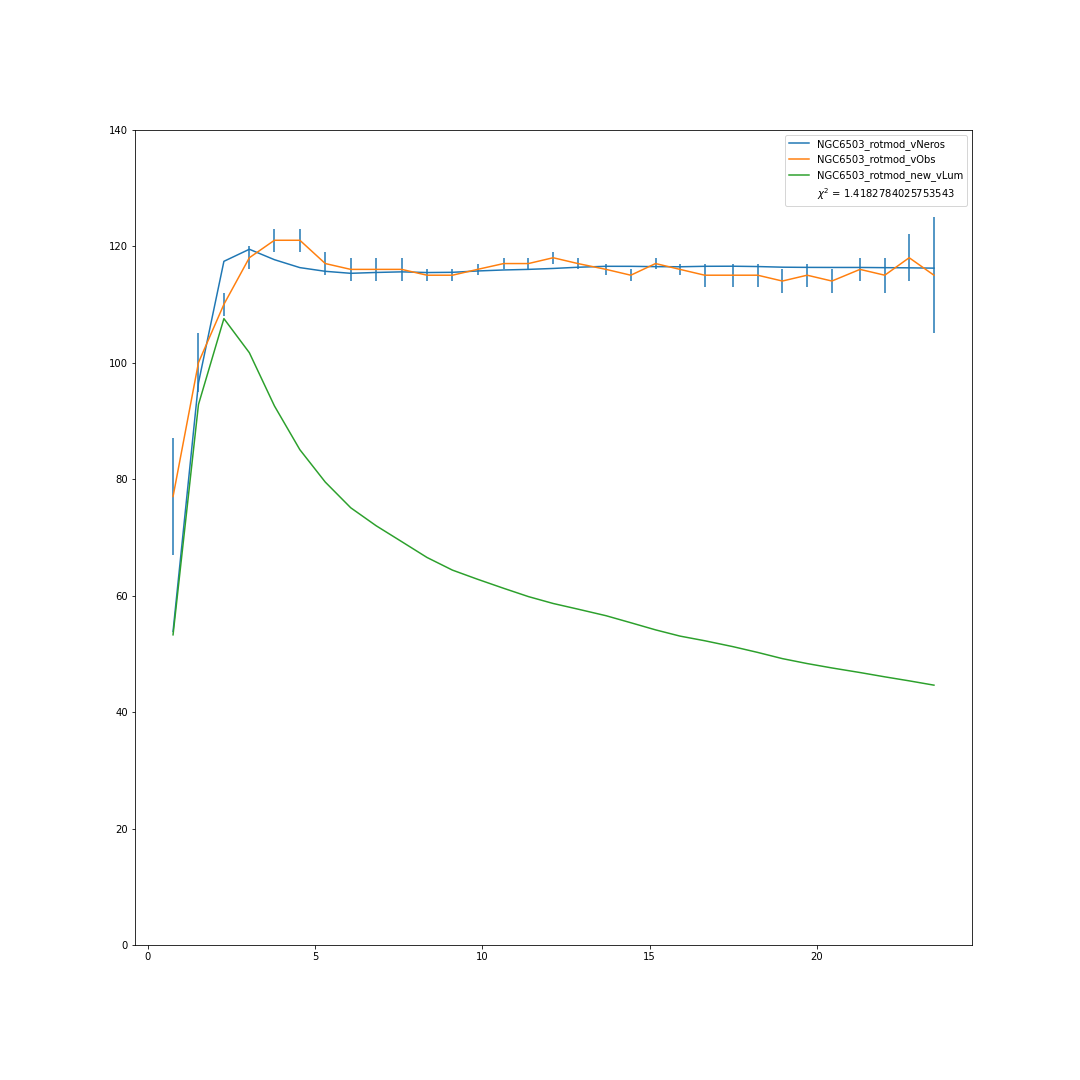
\includegraphics[width=0.95\linewidth]{figures/NGC6503_rotmod_XueSofue.png}
    \caption{Disk dominated NGC 6503} 
    \label{fig7:b} 
    \vspace{4ex}
  \end{subfigure} 
  \begin{subfigure}[c]{0.5\linewidth}
    \centering
    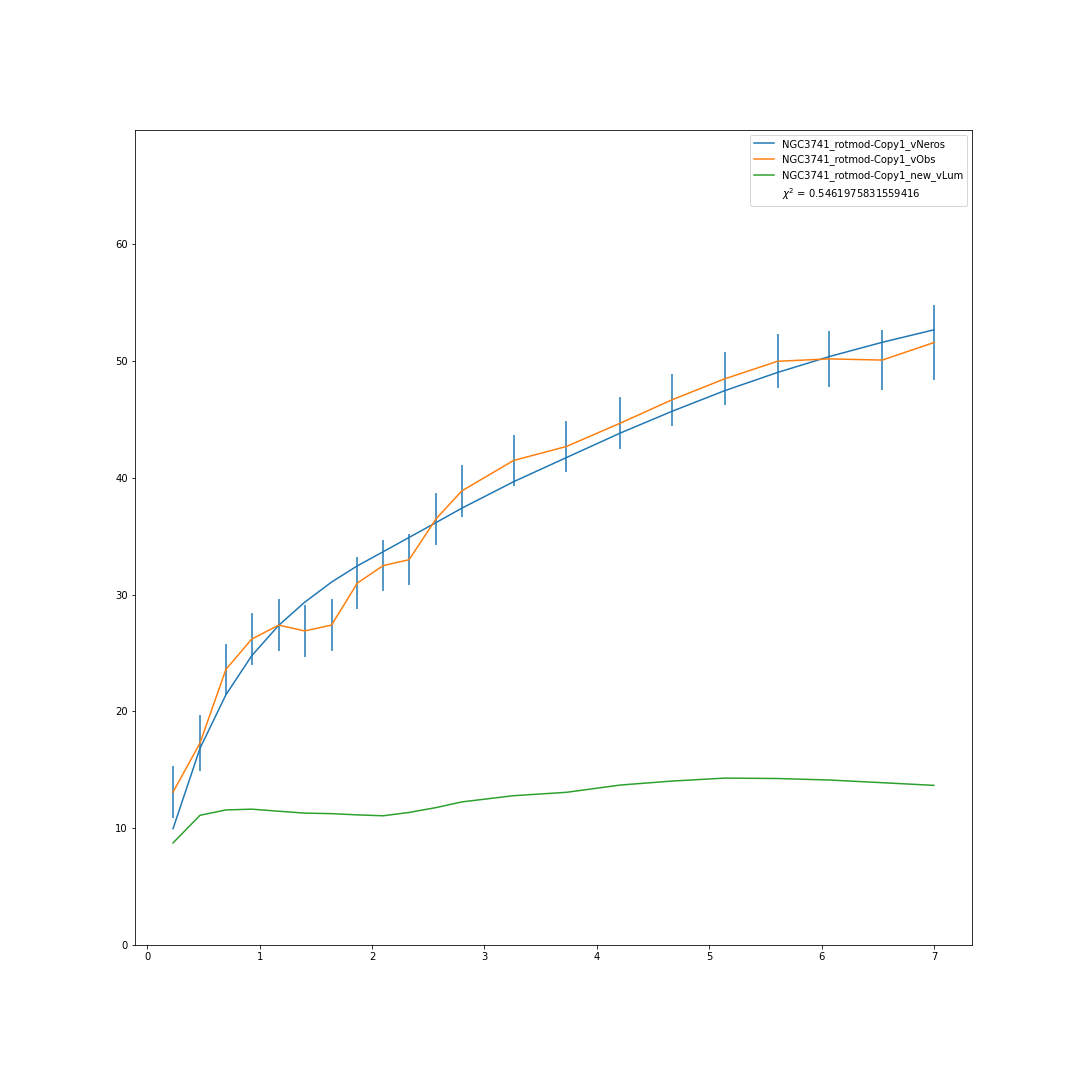
\includegraphics[width=0.95\linewidth]{figures/NGC3741_rotmod-Copy1_XueSofue.png} 
    \caption{Gas dominated NGC 3741} 
    \label{fig7:c} 
  \end{subfigure}%%
  \caption{Examples of range of spiral galaxy densities and RCFM rotation curve fits, points with error bars are the rotation curve data, Combined baryonic models are represented by the green lines, and the RCFM fit is the blue line. (YO BLUE : NOTE: remove orange lines, fit through data distracts from our fit)  }
  \label{fig7} 
\end{figure*}
 
 
    
%%%%%%%%%%%%%%%%%%%%%%%%%%%%%%%%%%%%%%%%%%%%%%%%%%%%%%%%%%%%%%%%%%%%%%%%%%%%%%%%%%%%%%%%%%%%%%%%%%%%%%%%%%%%%%%%%%%%%%%%%%%%%%%%%%%%%%%%%%%%%%%%%%%%%%%%%%%%%%%%%%%%%%%%%%%%%%%%%%%%%%%%%%%%%%%%%%%%%%%%%%%%%%%%%%%%%%%%%%%%%%%%%%%%%%%%%%%%%%%%%%%%%%%%%%%%%%%%%%%%%%%%%%%%%%%%%%%%%%%%%%%%%%%%%%%%%%%%%%%%%%%%%%%%%%%%%%%%%%%%%%%%%%%%%%%%%%%%%%%%%%%%  
    
     

\bibliography{LCM} 

\end{document}
%
% ****** End of file apssamp.tex ******